%%
%% Copyright 2007, 2008, 2009 Elsevier Ltd
%%
%% This file is part of the 'Elsarticle Bundle'.
%% ---------------------------------------------
%%
%% It may be distributed under the conditions of the LaTeX Project Public
%% License, either version 1.2 of this license or (at your option) any
%% later version.  The latest version of this license is in
%%    http://www.latex-project.org/lppl.txt
%% and version 1.2 or later is part of all distributions of LaTeX
%% version 1999/12/01 or later.
%%
%% The list of all files belonging to the 'Elsarticle Bundle' is
%% given in the file `manifest.txt'.
%%

%% Template article for Elsevier's document class `elsarticle'
%% with numbered style bibliographic references
%% SP 2008/03/01
%%
%%
%%
%% $Id: elsarticle-template-num.tex 4 2009-10-24 08:22:58Z rishi $
%%
%%
\documentclass[preprint,5p,twocolumn,12pt]{elsarticle}

%% Use the option review to obtain double line spacing
%% \documentclass[preprint,review,12pt]{elsarticle}

%% Use the options 1p,twocolumn; 3p; 3p,twocolumn; 5p; or 5p,twocolumn
%% for a journal layout:
%% \documentclass[final,1p,times]{elsarticle}
%% \documentclass[final,1p,times,twocolumn]{elsarticle}
%% \documentclass[final,3p,times]{elsarticle}
%% \documentclass[final,3p,times,twocolumn]{elsarticle}
%% \documentclass[final,5p,times]{elsarticle}
%% \documentclass[final,5p,times,twocolumn]{elsarticle}

%% if you use PostScript figures in your article
%% use the graphics package for simple commands
%% \usepackage{graphics}
%% or use the graphicx package for more complicated commands
%% \usepackage{graphicx}
%% or use the epsfig package if you prefer to use the old commands
%% \usepackage{epsfig}

%% The amssymb package provides various useful mathematical symbols
\usepackage{amssymb}
\usepackage{graphicx}

\usepackage[section]{placeins}
\usepackage{colortbl}
\usepackage{longtable}

\usepackage{natbib}
\usepackage{multirow}
\usepackage{fancybox}
%\usepackage[T1]{fontenc}
\usepackage[ansinew]{inputenc}
%\usepackage{a4wide, url}

\usepackage[normalem]{ulem}
%\newlength\wvtextpercent
%\setlength\wvtextpercent{0.009\textwidth}
\usepackage{latexsym}
\usepackage[draft]{fixme}
\usepackage{verbatim}
\usepackage{listings}
\usepackage{amsmath}

\usepackage{array} % and/o
\usepackage{hyperref}
\usepackage{breakurl}
\usepackage{url}
\usepackage{xspace}
%% The amsthm package provides extended theorem environments
%% \usepackage{amsthm}

%% The lineno packages adds line numbers. Start line numbering with
%% \begin{linenumbers}, end it with \end{linenumbers}. Or switch it on
%% for the whole article with \linenumbers after \end{frontmatter}.
%% \usepackage{lineno}

%% natbib.sty is loaded by default. However, natbib options can be
%% provided with \biboptions{...} command. Following options are
%% valid:

%%   round  -  round parentheses are used (default)
%%   square -  square brackets are used   [option]
%%   curly  -  curly braces are used      {option}
%%   angle  -  angle brackets are used    <option>
%%   semicolon  -  multiple citations separated by semi-colon
%%   colon  - same as semicolon, an earlier confusion
%%   comma  -  separated by comma
%%   numbers-  selects numerical citations
%%   super  -  numerical citations as superscripts
%%   sort   -  sorts multiple citations according to order in ref. list
%%   sort&compress   -  like sort, but also compresses numerical citations
%%   compress - compresses without sorting
%%
%% \biboptions{comma,round}

% \biboptions{}

\newcommand{\eg}{e\@.g\@.~}                     % e.g.
\newcommand{\ie}{i\@.e\@.~}                     % i.e.
\newcommand{\cf}[1]{{\it cf.~#1}}
\newcommand{\etal}{\textit{et al.}\xspace}
\newcommand{\viz}{\textit{viz.}\xspace}
\newcommand{\quotes}[1]{``#1''}
\newcommand{\apriori}{\textit{a priori}\xspace}
\newcommand{\adhoc}{\textit{ad hoc}\xspace}
\newcommand{\eat}[1]{}

\newcommand{\superscript}[1]{\ensuremath{^{\textrm{#1}}}}
\newcommand{\subscript}[1]{\ensuremath{_{\textrm{#1}}}}
\newcommand{\Time}{\mathbb{T}}

\newcommand{\iri}{\textsc{iri}\xspace}
\newcommand{\dtwor}{\textsc{d2r}\xspace}
\newcommand{\rtwoo}{\textsc{r\subscript{2}o}\xspace}
\newcommand{\stwoo}{\textsc{s\subscript{2}o}\xspace}
\newcommand{\bigstwoo}{\textsc{S\subscript{2}O}\xspace}
\newcommand{\odemapster}{\textsc{odemapster}\xspace}
\newcommand{\owl}{\textsc{owl}\xspace}
\newcommand{\rdf}{\textsc{rdf}\xspace}
\newcommand{\csparql}{\textsc{c-sparql}\xspace}
\newcommand{\sparql}{\textsc{sparql}\xspace}
\newcommand{\spasql}{\textsc{spasql}\xspace}
\newcommand{\sparqlstr}{\textsc{sparql}\subscript{Stream}\xspace}
\newcommand{\sql}{\textsc{sql}\xspace}
\newcommand{\stream}{\textsc{stream}\xspace}
\newcommand{\snee}{\textsc{snee}\xspace}
\newcommand{\sneeql}{\textsc{snee}ql\xspace}
\newcommand{\uri}{\textsc{uri}\xspace}
\newcommand{\xml}{\textsc{xml}\xspace}

\newcommand{\streamingsparql}{\textsc{s}treaming\textsc{sparql}\xspace}
\newcommand{\cql}{\textsc{cql}\xspace}
\newcommand{\dtworq}{\textsc{d2rq}\xspace}

\newcommand{\gav}{GAV\xspace}
\newcommand{\lav}{LAV\xspace}
\newcommand{\dsms}{DSMS\xspace}
\newcommand{\dbms}{DDMS\xspace}



%%%%%%%%%%%%%%%%%%%%%%%%%%%%%%%%%%%%%%%%%%%%%%%%%%%%%%%%%%%%%%%%%%%%%%



%%%%%%%%%%%%%%%%%%%%%%%%%%%%%%%%%%%%%%%%%%%%%%%%%%%%%%%%%%%%%%%%%%%%%%
%%%% Listing styles

\lstset{numberbychapter=false}
\lstset{captionpos=b}
\lstset{frame=none}
\lstset{breaklines=true}

% R2O
\lstdefinelanguage{R2O}{
morekeywords={streamschema,desc,name,has,stream,streamType,documentation,timestamp, keycol,nonkeycol,columnType,conceptmap,def,uri,as,virtualStream,described,by,
attributemap,has,column,applies,if,operation,dbrelationmap,toConcept,joins,via,condition},
sensitive=true,%
morecomment=[l]\#,%
morestring=[b]',%
}
\lstdefinestyle{R2OStyle}{basicstyle=\sffamily\scriptsize,
                        %keywordstyle=\lstuppercase,
                        emphstyle=\itshape,
                        showstringspaces=false,
                        tabsize=2,
                        }

% SNEEql
\lstdefinelanguage{SNEEql}[]{SQL}{
                        morekeywords={RSTREAM,ISTREAM,DSTREAM,TO,SLIDE}
}
\lstdefinestyle{SNEEqlStyle}{basicstyle=\ttfamily\scriptsize,
                        %keywordstyle=\lstuppercase,
                        emphstyle=\itshape,
                        showstringspaces=false,
                        }

%SPARQL_Stream
\lstdefinelanguage{SPARQLSTR}[]{SQL}{
morekeywords={STREAM, PREFIX, WINDOW, RANGE, SLIDE, AGGREGATE, AVG,
  STEP, REGISTER, GRAPH, FILTER, QUERY, HOURS, MINUTES, TO, NOW, RSTREAM, ISTREAM, DSTREAM},
sensitive=true,%
morecomment=[l]\#,%
morestring=[b]',%
}

\lstdefinestyle{SPARQLSTRStyle}{basicstyle=\sffamily\scriptsize,
                        %keywordstyle=\lstuppercase,
                        emphstyle=\itshape,
                        showstringspaces=false,
                        tabsize=4,
                        }
%%%%%%%%%%%%%%%%%%%%%%%%%%%%%%%%%%%%%%%%%%%%%%%%%%%%%%%%%%%%%%%%%%%%%%


\journal{JWS special issue on Web-scale Semantic Information Processing}

\begin{document}

\begin{frontmatter}

%% Title, authors and addresses

%% use the tnoteref command within \title for footnotes;
%% use the tnotetext command for the associated footnote;
%% use the fnref command within \author or \address for footnotes;
%% use the fntext command for the associated footnote;
%% use the corref command within \author for corresponding author footnotes;
%% use the cortext command for the associated footnote;
%% use the ead command for the email address,
%% and the form \ead[url] for the home page:
%%
%% \title{Title\tnoteref{label1}}
%% \tnotetext[label1]{}
%% \author{Name\corref{cor1}\fnref{label2}}
%% \ead{email address}
%% \ead[url]{home page}
%% \fntext[label2]{}
%% \cortext[cor1]{}
%% \address{Address\fnref{label3}}
%% \fntext[label3]{}

\title{Querying Streaming Data Sources through Ontology Mappings :p put title here}

%% use optional labels to link authors explicitly to addresses:
%% \author[label1,label2]{<author name>}
%% \address[label1]{<address>}
%% \address[label2]{<address>}

\author[rvt]{Jean-Paul Calbimonte\corref{cor1}}
\ead{jp.calbimonte@upm.es}
\author[rvt]{Oscar Corcho}
\ead{ocorcho@fi.upm.es}
\author[els]{Alasdair J. G. Gray}
\ead{a.gray@cs.man.ac.uk}

\cortext[cor1]{Corresponding author}

\address[rvt]{Ontology Engineering Group, Departamento de Inteligencia Artificial, \\ 
Facultad de Inform\'{a}tica, Universidad Polit\'{e}cnica de Madrid,\\ Campus de Montegancedo s/n 28660, Boadilla del Monte, Spain\\}
\address[els]{School of Computer Science, The University of Manchester,\\
Oxford Road, Manchester M13 9PL, United Kingdom}

\begin{abstract}
Ubiquitous and inexpensive networks of data capturing devices are being developed and deployed nowadays increasing the availability of streaming data sources for a number of applications and domains. 
%The availability of streaming data sources is progressively increasing thanks to the development of ubiquitous data capturing technologies such as sensor networks. 
The heterogeneity of these sources introduces the requirement of providing data access and query capabilities in a unified and coherent manner, whilst allowing users to express their needs at a conceptual level, independent of implementation and language-specific details. In this paper we describe an ontology-based streaming data access approach for overcoming this problem. Sources link their data content to ontologies through \stwoo declarative mappings. Users can query over these ontologies using \sparqlstr, an extension of \sparql for streaming data, and the translation algorithms generate the necessary queries in the underlying streaming data source. An implementation of the approach is also presented. With this proposal we expect to set the basis for future efforts in ontology-based streaming data integration.


\end{abstract}

\begin{keyword}
Streaming query processing\sep Ontology-based data access \sep Semantic query translation

%% keywords here, in the form: keyword \sep keyword

%% MSC codes here, in the form: \MSC code \sep code
%% or \MSC[2008] code \sep code (2000 is the default)

\end{keyword}

\end{frontmatter}

%%
%% Start line numbering here if you want
%%
% \linenumbers

%% main text
\section{Introduction}
\label{intro}
In recent years, advances in wireless sensor technologies and communications have opened the possibility of deploying large-scale and ubiquitous sensor networks capable of live data capture, processing and delivery.
 
%Recent advances in wireless communications and sensor technologies have opened the way for deploying networks of interconnected sensing devices capable of ubiquitous data capture, processing and delivery.
Deployments of sensor networks are expected to increase significantly in the upcoming years because of their advantages and unique features. Tiny and inexpensive devices can be installed virtually anywhere, execute elementary computations and still be reachable thanks to wireless communications. Therefore these devices can be used for a wide variety of applications including security surveillance, healthcare provision, traffic control and environmental monitoring.
In this context several challenges are raised for the research community, and the one we are concerned with is about accessing and querying the enormous amount of loosely structured data collected by these sensors. Client applications require a suitable platform to query data from sensors, streaming query engines or databases, in terms of a uniform schema that hides the diverse and internal data representations of each source.

As an example, consider a web application which aids an emergency planner to detect and co-ordinate the response to flood risk alerts in the coast of South East England. 
This involves retrieving relevant data from multiple sources, \eg meteorological forecasts from the Met Office (UK's National Weather Service)\footnote{\url{http://www.metoffice.gov.uk} accessed 15 September 2010.}, real-time wave and tide data from sensor networks deployed in the region by the \textsc{CCO} (Channel Coastal Observatory)\footnote{\url{http://www.channelcoast.org/} accessed 15 September 2010.}, and any other relevant sources of data such as the \textsc{NFCDD} (Environment Agency's\footnote{\url{http://www.environment-agency.gov.uk/} accessed 15 September 2010.} National Flood and Coastal Defence Database)  providing
data about coastal defences. 
Typically sources are managed autonomously and model their data according to the needs of the deployment. 
To integrate the data requires linking the sources to a common data model so that conditions that are likely to cause a flood can be detected using prediction models, and presented to the user in terms of their domain, \eg flood risk assessment. \\
%As an example, consider a web application which aids an emergency planner to detect and co-ordinate the response to a forest fire in Spain. 
%This involves retrieving relevant data from multiple sources, \eg weather data from \textsc{aemet} (Agencia Espa\~nola de Meteorolog\'ia)\footnote{\url{http://www.aemet.es} accessed 15 September 2010.}, sensor data from sensor networks deployed in the region, and any other relevant sources of data such as the \textsc{esa} satellite imagery providing fire risks\footnote{\url{http://dup.esrin.esa.int/ionia/wfa/index.asp} accessed 15 September 2010.}. 
%Typically sources are managed autonomously and model their data according to the needs of the deployment. 
%To integrate the data requires linking the sources to a common data model so that conditions that are likely to cause a fire can be detected, and presented to the user in terms of their domain, \eg fire risk assessment. 

%In the context of the Semantic Web vision, several initiatives that aim at providing semantic access to traditional (stored) data sources have been launched in the past years.

We propose that ontologies can be used as such a common model as it has been done in the past for other types of data sources (\eg relational \cite{Wache_01}) . 
For the scenario presented here, we use a network of ontologies that includes and extends ontologies from \textsc{sweet}\footnote{\url{http://sweet.jpl.nasa.gov/} accessed 15 September 2010.} and the W3C incubator group's semantic sensor network ontology.
\footnote{\url{http://www.w3.org/2005/Incubator/ssn/wiki/Semantic_Sensor_Network_Ontology} accessed 15 September 2010.}
%However, such a scenario requires techniques for ontology-based access to streaming data sources.

The work presented in this paper considers advances done by the semantic web and database communities over the last decade. On the one hand, the semantic web research has produced mapping languages and software for enabling ontology-based access to stored data sources, \eg \rtwoo \cite{Barrasa_04} and \dtworq \cite{Bizer_07}.
These systems provide semantic access to traditional (stored) data sources by providing mappings between the elements in the relational and ontological models \cite{Sahoo_09}.
However, similar solutions for streaming data mapping and querying using ontology-based approaches have not been explored yet.

On the other hand, the database research community have investigated data stream processing where the data is viewed as an append-only sequence of tuples.
Systems such as \stream \cite{Arasu_06a} and Borealis \cite{Abadi_2005} have focused on query evaluation and optimization over streams with high, variable, data rates.
Other systems such as \snee \cite{Galpin_09} and TinyDB \cite{Madden_05}, have focused on data generated by sensor networks, which tends to be at a lower rate, and query processing in the sensor network where resources are more constrained and energy efficiency is the primary concern.
There have also been proposals for query processing over streaming \rdf data \cite{Bolles_08,Barbieri2010An-Execution-En}.
However there is still no bridging solution that connects these technologies coherently in order to answer the requirements of %
\begin{itemize}
\item i)~establishing mappings between ontological models and streaming data source schemas. 
\item ii)~accessing streaming data sources through queries over ontology models.
\end{itemize}
%


In this paper we focus on providing ontology-based access to streaming data sources, including sensor networks, through declarative continuous queries.
We build on the existing work of \rtwoo for enabling ontology-based access to relational data sources, and \snee for query evaluation over streaming and stored data sources.
This constitutes a first step towards a framework for the integration of distributed heterogeneous streaming and stored data sources through ontological models. %and to the provision of Linked Data for streams~\cite{LePhuoc_09,Page_09,Sequeda_09}.
%\fxnote{AG: Can we drop the last clause of the sentence to do with Linked Data? I'm not convinced it adds to our argument.}
In Section~\ref{sec:background} we provide more detailed descriptions of \rtwoo and stream query processing in order to present the foundations of our approach in Section~\ref{approach}. 
In Section~\ref{syntax} we present the syntactic extensions for \sparql to enable queries over \rdf streams, and present \stwoo for stream-to-ontology mappings. 
The semantics of these extensions are detailed in Section~\ref{semanticsstreaming} and a first implementation of the execution of the streaming data access approach is explained in Section~\ref{execution}.
Related work is discussed in Section \ref{sec:related-work} and our conclusions in Section~\ref{conclusions}. 


%%% Local Variables: 
%%% mode: latex
%%% TeX-master: "rere"
%%% End: 


\section{Preliminaries}
\label{sec:background}

This section describes the existing work upon which our approach is based, \ie ontology-based data access and querying through mappings, and data access for streaming data.
A full discussion of related work can be found in Section~\ref{sec:related-work}.


\subsection{Ontology-based Access to Stored Relational Data}
\label{sec:ontol-based-access-stored}

The goal of ontology-based data access is to generate semantic web content from existing relational data sources available on the web \cite{Sahoo_09}.
The objective of systems following this approach is to allow users to construct queries over an ontology (\eg using a query language as \sparql), which are then rewritten into a set of queries expressed in the query language of the data source (typically \sql), according to the specified mappings.
The query results are then converted back from the relational format into \rdf, which is returned to the user.
\odemapster is one such system which uses the \rtwoo (Relational-to-Ontology) language to express the mappings between the relational data source and the ontology \cite{Barrasa_04}.

The mapping definition language \rtwoo defines relationships between a set of ontologies and relational schemas \cite{Barrasa_04}.
%The resulting mappings are saved as \xml which enables them to be independent of any specific DBMS or ontology language.
\rtwoo\ specifically considers classes, object and datatype properties in an ontology. They are described in terms of selections and transformations over database relations following a Global-as-View (\gav) approach \cite{Lenzerini_02}, and can be created either manually or with the help of a mapping tool\footnote{\url{http://www.neon-toolkit.org/wiki/ODEMapster} accessed 29 September 2010.}.
\rtwoo\ covers a wide set of mapping cases common in relational database to ontology situations: %\rtwoo\ is designed to cope with the following mapping cases:
\begin{itemize}
\item A database table maps to one class in the ontology. Then the table columns map to attributes or relations of the concept. For each row in the table a corresponding instance in the ontology will be generated, with its attribute values filled with the columns data.
\item A single database table is mapped to more than one class in the ontology, and for each row a single instance of each class is generated. %In this case some columns will be mapped to a concept attributes while other columns will be mapped to other concept attributes.
\item A single database table is mapped to more than one class in the ontology, and multiple instances can be generated for each class. It is a more general case than the previous one; multiple instances of the same ontology concept can be generated from a single database record.
\end{itemize}

Mapping relations to ontologies often requires performing operations on the relational sources.
Several cases are handled by \rtwoo and detailed below.
\begin{description}
\item[Direct Mapping.] A single relation maps to an ontology class and the attributes of the relation are used to fill the property values of the ontology instances. Each row in the relation will generate a class instance in the ontology.
\item[Join/Union.] A single relation does not correspond alone to a class, but it has to be combined with other relations. The result of the join or union of the relations will generate the corresponding ontology instances.
\item[Projection.] Not all the attributes of a relation are always required for the mapping. The unnecessary attributes can simply be ignored. In order to do so, a projection on the needed attributes can be performed.
\item[Selection.] Not all rows of a relation correspond to instances of the mapped ontology class. A subset of the rows must be extracted. To do so, selection conditions can be applied to choose the desired subset for the mapping.
\end{description}
It is possible to combine joins, unions, projections and selections for more complex mapping definitions.
\rtwoo also enables the application of functions, \eg concatenation, sub-string, or arithmetic functions, to transform the relational data into the appropriate form for the ontology.



\subsection{Relational Data Streams}
\label{sec:query-relat-streams}

A relational data stream is an append only, potentially infinite, sequence of timestamped tuples \cite{Golab2003Issues-in-data-}, examples of which include stock market tickers, heart rate monitors, and sensor networks deployed to monitor the environment.
Data streams can be classified into two categories:
\begin{description}
\item[Event-streams.] A tuple is generated each time an event occurs, \eg the sale of shares, and can have variable, potentially very high, data rates.
\item[Acquisitional-streams.] A tuple is measured at a predefined regular interval, \eg the readings made by a sensor network.
\end{description}
Users are typically interested in being informed continuously about the most recent stream values, with older tuples being less relevant.
Classical database query processing is not adequate since data must first be stored and then queried with one-off evaluation.
Hence, query languages \cite{Brenninkmeijer_08,Arasu_2006} and data stream management systems (DSMS) \cite{Arasu_06a,Abadi_2005,Galpin_09,Madden_05} have been developed to process continuous long-lived queries over data streams as tuples arrive.

One existing approach is \sneeql, which has a well defined, unified semantics for declarative expressions of data needs over event-streams, acquisitional-streams, and stored data \cite{Brenninkmeijer_08}.
\sneeql can be viewed as extending \sql for processing data streams.
The main additional constructs of relational streaming query languages are explained below. and we present them using the \sneeql syntax. 
\begin{description}
\item[Window.] A window over a data stream transforms the infinite sequence of tuples into a bounded bag of tuples over which traditional relational operators can be applied. A window is specified as: 
\begin{align*}
\textsf{\small{FROM}}\ {start}\ \textsf{\small{TO}}\ {end}\ [\textsf{\small{SLIDE}}\ {int}\ {unit}]
\end{align*}
Where ${start}$ and ${end}$ are of the form `$\textsf{\small{NOW}} - {literal}$' and define the range of the window with respect to the evaluation time. The optional \textsf{\small{SLIDE}} parameter specifies how often windows are evaluated.

\item[Window-to-Stream.] Window-to-stream operators are used to convert a stream of windows into a stream of tuples. \sneeql supports three such operators: \textsf{\small{RSTREAM}} for all tuples appearing in the window, \textsf{\small{ISTREAM}} for tuples that have been added since the last window evaluation, and \textsf{\small{DSTREAM}} for tuples that have been deleted since the last window evaluation.
\end{description}
%Queries expressed in the \sneeql language are optimized for evaluation within a sensor network over acquisitional-streams by the \snee compiler \cite{Galpin_09}. \snee has recently been extended to enable query evaluation over event-streams either within the sensor network (in-network query processing) or on computational hardware outside of the sensor network.



%%% Local Variables: 
%%% mode: latex
%%% TeX-master: "rere"
%%% End: 

%

\subsection{Ontology-based data integration}
\label{obdi}
%- focus on integration problems

Data integration can be defined as the process of providing unified and transparent data access to multiple and heterogeneous data sources [Len02]. The problem of integrating heterogeneous data sources involves not only providing access to information but also providing means of interpreting and processing the data in a consistent manner. When dealing with different sources it is often complicated to establish the meaning of the incoming data. And if the meaning cannot be clearly identified, then it is impossible to pair information for the different sources [RAY+00]. Problems of this kind are mainly due to confusion in term meanings and naming conflicts. Added to syntactical conflicts, the semantic integration challenge is hard to tackle.
We can identify the main issues of data integration as [WVV+01]:
\begin{itemize}
	\item Incompatibility in communication and protocols, across different data management systems
	\item Syntactical heterogeneity: differences in data model representation and structure, incompatibility of data values.
	\item Semantic heterogeneity: differences in naming and abstraction level, homonyms and synonyms in schemas.
\end{itemize}.
Ontologies provide a means of explicitly specifying the meaning of the information that will be interchanged between systems. In that way it can help achieve semantic interoperability: regardless of the source's data syntax or semantics, we can map it to a known ontology and access the data in terms of the mediated ontological view [WVV+01]. As a consequence semantic declarative queries can be written in terms of the mediated schema.
It has been acknowledged that ontologies may be useful to solve this semantic heterogeneity problem as it is described in [WVV+01, DH05]. We can mention several systems and prototypes based on ontologies for data integration support: OBSERVER [MIK+00], SIMS [ACH+93], Carnot [HJK+93], DWQ [CDL+98], PICSEL [GLR00], MOMIS [BBV+07].
The main role and purpose of ontologies in an integration system is to explicitly state the semantics of the data sources so that it can be possible to identify and establish semantic relationships between these sources. For instance, if a data source stores person information and another source stores student information, the ontology may represent both concepts, with person subsuming student. This information can later be exploited by query integrators to coherently perform joins or unions over these sources.
Data sources can be relational databases, data files, xml files or any other storing media. Most of the work on data integration has been centred on relational databases, as it is the most widespread way of storing large volumes of information. In any case the ultimate goal is to allow querying the different sources through a uniform interface, hiding the underlying heterogeneous schemas. Therefore the applications querying the integrated system must only focus on the information they wish to obtain, leaving to the integration system the work of searching for the information in the different sources, clearly simplifying the development of upper layer applications on top of the integration infrastructure.
Research on the subject has produced many approaches to building such integration systems. We mention two main alternatives: the \textit{virtualisation} and \textit{materialisation} approaches [IKK05].
In the virtualisation approach queries are posed over the mediated schema and a mediator component identifies the sources that will be needed to produce the answer. Then a series of appropriate sub-queries are automatically written for these sources and executed. The results of each source are retrieved, post-processed and transformed to the mediated schema and returned to the caller application.
This alternative allows answering queries on demand, even if the update rate of data is high and the queries are potentially arbitrary. As the queries are rewritten dynamically for each of the sources, it is possible to retrieve any portion of data exposed through the mediated schema. On the other hand the transformations on the queries and the processing of the data from the sources to the mediated schema may be complex and incur in performance issues. Another potential problem is data source availability, as the queries are performed live; if the source is unreachable then the queries may not be able to be completed. Even if the source is available, latency caused by networking or connection problems may increase the query response time.
The materialisation approach differs from the virtualised one in that it extracts and transforms the data from the sources periodically, instead of performing on-the-fly conversions each time a query is being executed. Instead, relevant data is first identified, and extracted from the multiple data sources in a batch process operation. The extracted data is then stored in a data warehouse where it can be accessed by the external applications. The data warehouse can then be updated periodically depending on the requirements. Under this approach, the time consumed in retrieving the data from the sources is moved to the off-line phase of updating the centralised data warehouse. Therefore when the external applications query the integration system, results can be accessed almost immediately. However the data may be stale in occasions, and it may not be possible to access all possible pieces of data, as the warehouse only stores selected materialised views of the original sources.
In the case of the virtualised approach, a mediator component is introduced as a major feature of the integration architecture. This mediator is in charge of transforming the original query into sub-queries for the sources and then transforming the results back to the mediated schema. This process of transformation is performed thanks to mapping definitions that establish relationships between the mediated and source schemas. 

There are three main alternatives for defining these mappings [Len02, IKK05]: \textit{Global-as-view (GAV)}, \textit{Local-as-view (LAV)} and a combination of both, \textit{GLAV}.
In the LAV approach, each of the source schemas is represented as a view in terms of the global schema. If our system $\mathcal{I}$ is represented as:
$\mathcal{I = <G,S,M>}$ , where $\mathcal{G}$ is the global schema, $\mathcal{S}$ is a source schema and $\mathcal{M}$ is the mapping between $\mathcal{G}$ and $\mathcal{S}$, then the mapping assertions in $\mathcal{M}$ will be a set of elements of the form:
$s \leadsto q_{\mathcal{G}}$
Where $s$ is an element of $\mathcal{S}$ and $q_{\mathcal{G}}$ is a query over the global schema $mathcal{G}$.
This approach is useful if the global schema is well established and if the sources suffer modifications constantly. Notice that changes in the sources do not affect the global schema. However, the query processing is not obvious, as it is not explicitly stated how to obtain the data in the mapping definition. Query rewriting techniques such as query answering using views can be used in this approach [Hal01]. Examples of LAV based works are DWQ [CDL+98], InfoMaster [GKD97], Information Manifold [Lev98], PICSEL [GLR00].
The other approach, GAV, defines the mappings in the opposite way. The global schema elements are represented as views over the source schemas. The mapping definition explicitly defines how to query the sources to obtain the desired information in terms of the global schema. Following the system representation $\mathcal{I = <G,S,M>}$, in the GAV approach the mapping assertions are elements of the form:
$g \leadsto q_{\mathcal{S}}$
Where $g$ is an element of the global schema $\mathcal{G}$ and is expressed as a view $q_{\mathcal{S}}$, a query on the source schema. The advantage is that the mapping itself already indicates how to query the sources to obtain the data, so the processor can directly use this information to perform the query rewriting. The main disadvantage is that in case of changes or additions on the sources -e.g. a new source is added- then the global schema may suffer changes and this may affect other mapping definitions. Examples of GAV based works are SIMS [ACH+93], TSIMMIS [GHI+97], Carnot [HJK+93], Gestalt [RS98], MOMIS [BBV+07], IBIS [CCDG+03], DIS@DIS [CDL+03].
For the sake of completeness we can mention the GLAV (Global-Local-as-view) approach, which is a generalisation of the previous two. This formalism allows more expressive mappings than LAV and GAV combined, and it has been shown to reach the limits of tractability of these description languages [FLM99].

\section{Ontology-based Streaming Data Access}
\label{approach}
% lightweight description, architecture
% include graphic
% contributions

Querying streaming data and ontology-based access to stored data sources have already been studied by the research
community and concrete proposals and software have been produced to deal with them. However there is still no bridging
solution that allows connecting these technologies coherently in order to answer the requirements of i) establishing
mappings between ontological models and streaming data source schemas, and ii) accessing streaming data sources through
queries over ontology models.

%\begin{itemize}
%\item establishing mappings between global ontological models and streaming data source schemas.
%\item accessing streaming data sources through queries over ontology global models.
%\item integrating streaming and stored data sources through an ontological unified view.
%\item combining data from event-based streams and/or sensor networks acquisitional streams considering time and tuple windows.
%\item considering quality-of-service requirements for query optimisation and source selection during the integration.
%\end{itemize}

\begin{figure}[here]
%\vspace{-20pt} \hspace{20pt}
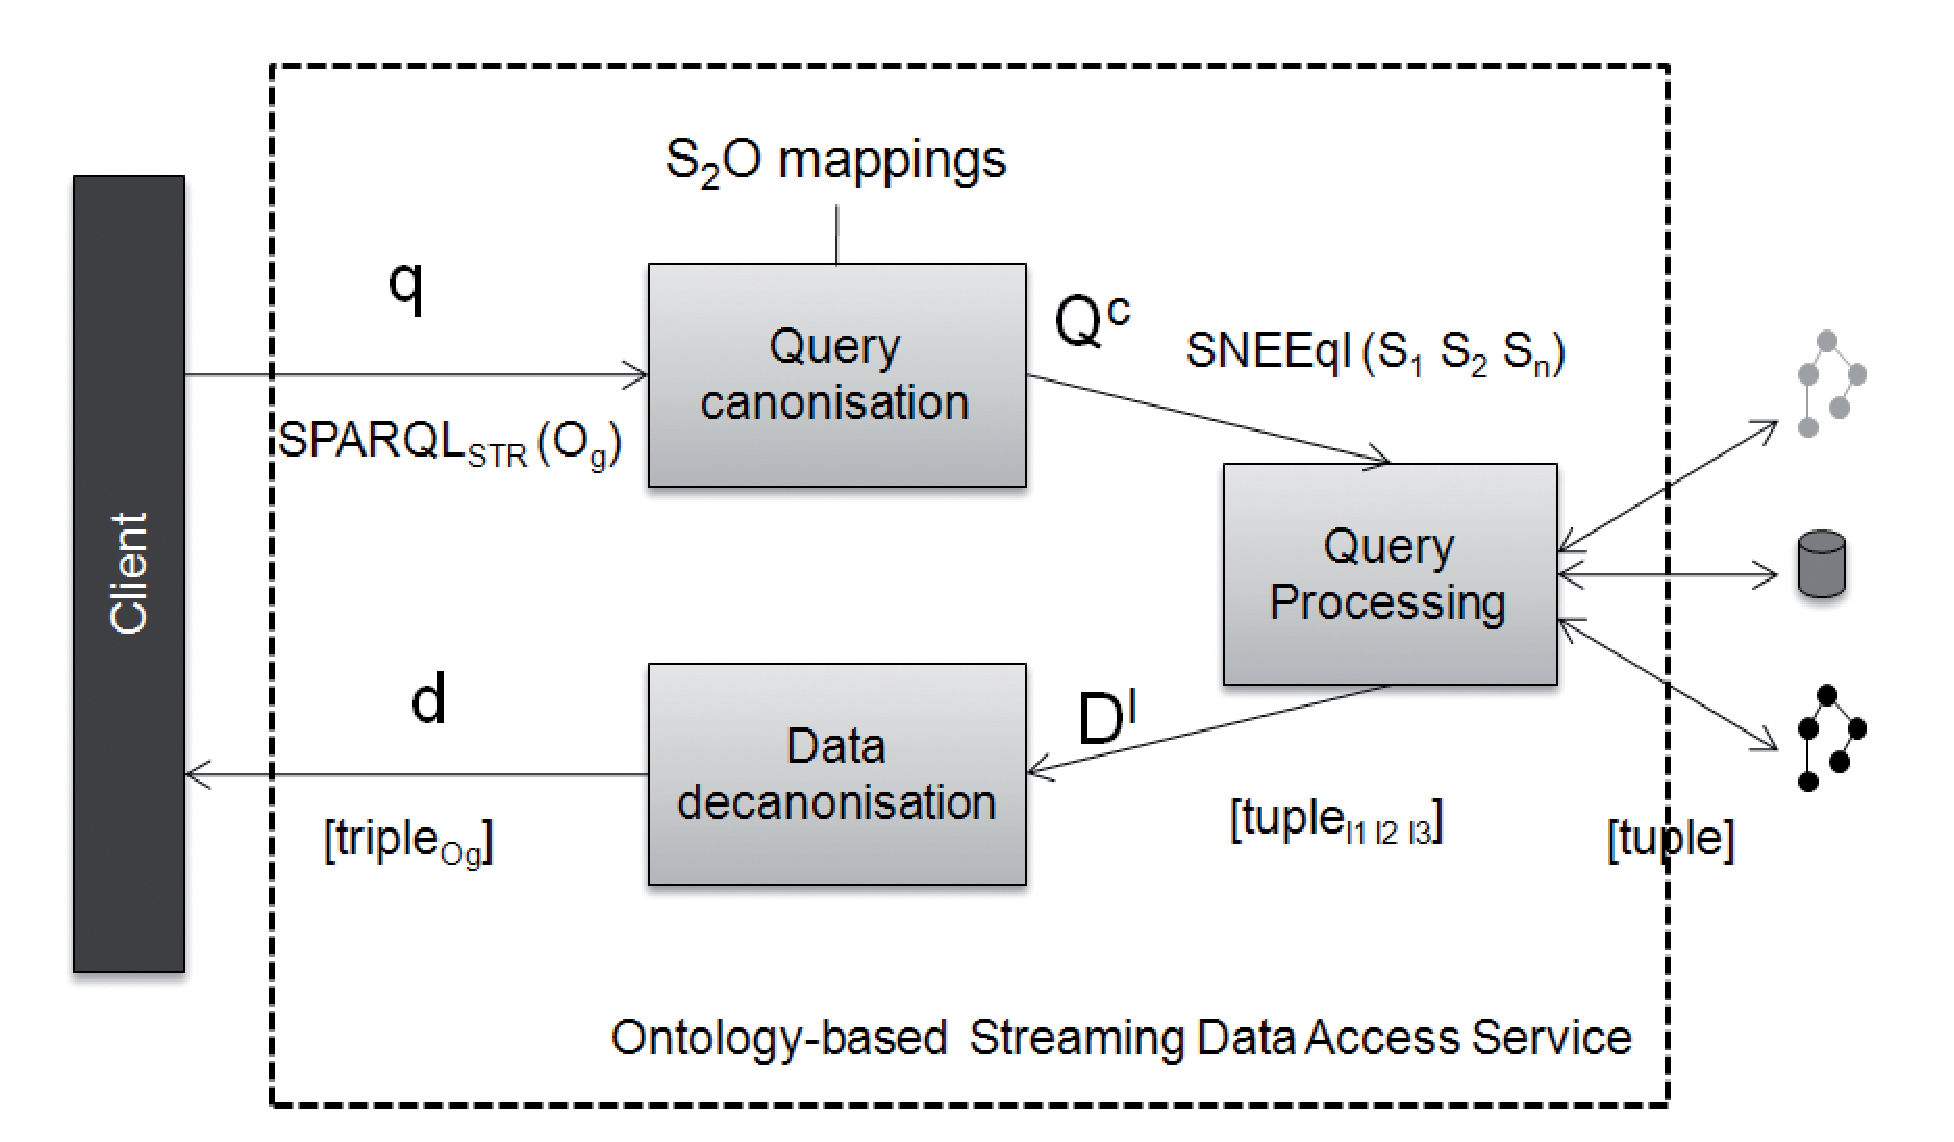
\includegraphics[width=8 cm]{img/approach}
%\vspace{-10pt} 
\caption{Ontology-based Streaming Data Access service} \label{fig:SemanticIntegrator} 
%\vspace{-10pt}
\end{figure}

Our approach consists in creating an Ontology-based Streaming Data Access service, depicted in Fig~\ref{fig:SemanticIntegrator}.\ %  that can receive requests over an ontological view and transforms them into queries for acquisitional or event-based stream sources or stored sources. The results of these queries can be integrated following a query plan and returned as RDF triples in terms of the global ontology. The approach is depicted in Fig ~\ref{fig:SemanticIntegrator}.
The service receives queries specified in terms of the classes and properties\footnote{We use the OWL nomenclature of
classes and object and datatype properties for naming ontology elements.} of the ontology using extensions of SPARQL
that support operators over RDF streams and windows (\sparqlstr, see the Streaming Extensions to SPARQL section). %\ref{streamingsparqlsyntax}). 
Then in order to transform the query in terms of the ontology into queries in terms of the sources, a set of mappings must be
specified. These mappings are based on the \rtwoo\ mapping language, which has been extended to support  streaming
queries and data, most notably window and stream operators (see the Streaming Extensions to \rtwoo\ section).%~  Section \ref{streamingr2osyntax}). 
This transformation process is called \textit{query canonisation}, and the target is a continuous query language (e.g. SNEEql), that is
expressive enough to deal with both streaming and stored sources, and to apply window, aggregates and window-to-stream
operations.

After the continuous query has been generated, the query processing phase starts, and the processor will deploy distributed query processing techniques~\cite{Kossmann_00} to extract the relevant data from the sources and perform the required joins, etc.\ %creating a query plan that indicates how the sources will be accessed and how the data will be joined and combined using the available operators\cite{Kossmann_00}.
%
Note that the execution in sources such as sensor networks may include in-network query processing, pull or push based data delivery and other data source specific settings. The result of the query processing will be a set of tuples that will be passed to a \textit{data decanonisation} process, which will transform these tuples to ontology instances.

As it can be seen, this approach requires several contributions and extensions to the existing technologies for continuous data querying, ontology-based data access and SPARQL query processing. This work focuses on a first stage that includes the process of transforming the SPARQL extended queries into queries over the streaming data sources using a language such as SNEEql as the target. In the next sections a description of the query and mapping extensions syntax and semantics will be detailed, and afterwards we will provide details of an implementation of this approach.

\section{Query and Mapping Syntax}
\label{syntax}

In this section we introduce the \sparqlstr query language, an extension to \sparql for streaming \rdf data, which has been inspired by previous proposals such as \csparql \cite{Barbieri2010An-Execution-En} and \sneeql \cite{Brenninkmeijer_08}.
However, significant improvements have been made that correct the types supported and the semantics of windowing operations, which can be summarized as: %
(i)~we only support windows defined in time, %
(ii)~the result of a window operation is a window of triples, not a stream, over which traditional operators can be applied, as such we have added window-to-stream operators, and %
(iii)~we have adopted the \sparql1.1 definition for aggregates.
We also present \stwoo for the definition of stream-to-ontology mappings.

\subsection{SPARQL\subscript{Stream}}
\label{streamingsparqlsyntax}

Just as in \csparql we define an \emph{\rdf stream} as a sequence of pairs $(T_i,\tau_i)$ where $T_i$ is an \rdf triple $\langle s_i,p_i,o_i \rangle$ and $\tau_i$ is a timestamp which comes from a monotonically non-decreasing sequence.
An \rdf stream is identified by an \iri, which provides the location of the data source\footnote{Note in our work the \iri 's identify virtual \rdf streams since they are derived from the streaming data sources.}.

Window definitions are of the form `\textsf{\small{FROM}} \textit{Start} \textsf{\small{TO}} \textit{End}  [\textsf{\small{STEP}}] [\textit{Literal}]', where the \textit{Start} and \textit{End} are of the form \textsf{\small{NOW}} or \textsf{\small{NOW}} � \textit{Literal}, and \textit{Literal} represents some number of time unit (\textsf{\small{DAYS}}, \textsf{\small{HOURS}}, \textsf{\small{MINUTES}}, or \textsf{\small{SECONDS}})\footnote{Note that the parser will also accept the non-plural form of the time units and is not case sensitive.}. 
The optional \textsf{\small{STEP}} indicates the gap between each successive window evaluation.
Note, if the size of the step is smaller than the range of the window, then the windows will overlap, if it coincides with the size of the window then every triple will appear in one and only one window, and if the step is larger than the range then the windows \emph{sample} the stream.
Also note that the definition of a window can be completely in the past.
This is useful for correlating current values on a stream with values that have previously occurred.

The result of applying a window over a stream is a timestamped bag of triples over which conjunctions between triple patterns, and other \quotes{classical} operators can be evaluated.
Windows can be converted back into a stream of triples by applying one of the window-to-stream operators in the \textsf{\small{SELECT}} clause: \textsf{\small{ISTREAM}} for returning all newly inserted answers since the last window, \textsf{\small{DSTREAM}} for returning all deleted answers since the last window, and \textsf{\small{RSTREAM}} for returning all answers in the window.

The additional grammar rules for expressing windows and window-to-stream operators can be found in Figure~\ref{fig:sparql-str-syntax}\footnote{Note that the parser will also accept the non-plural form of the time units and is not case sensitive.}.

 \begin{lstlisting}[style=R2OStyle,language=R2O,frame=none]%[upquote=true]
 SelectStrClause \longrightarrow 'SELECT' [WindowToStream] VariableList
 \end{lstlisting}

 \begin{figure}[t]
   \centering
   \scriptsize
   \begin{align*}
     {SelectStrClause} \longrightarrow&\ `\textsf{SELECT}'\ [{WindowToStream}]\ {VariableList}\\
     {WindowToStream} \longrightarrow&\ \textsf{`RSTREAM'} \mid \textsf{`ISTREAM'} \mid \textsf{`DSTREAM'}\\
     \\
     {FromStrClause} \longrightarrow&\ `\textsf{FROM}'\ [`\textsf{NAMED}']\ `\textsf{STREAM}'\ {StreamIRI} [{Window}]\\
     {Window} \longrightarrow&\ `[\textsf{FROM'}\ {TimeExp}\ {TimeUnit}\ `\textsf{TO'}\ {TimeEx}\ [{TimeUnit}]\ [`\textsf{STEP'}\ {Number}\ [{TimeUnit}]]`]'  \mid\\
     & `[\textsf{NOW}\ [`\textsf{STEP'}\ {Number}\ [{TimeUnit}]]`]']'\\
     {TimeExp} \longrightarrow&\ `\textsf{NOW'}\ [`-'\ {Number}]\\
     {TimeUnit} \longrightarrow & \textsf{`SECONDS'} \mid \textsf{`MINUTES'} \mid \textsf{`HOURS'} \mid \textsf{`DAYS'} 
   \end{align*}
   \caption{Additional grammar rules for window and window-to-stream constructs of \sparqlstr.}
   \label{fig:sparql-str-syntax}
 \end{figure}
Listing~\ref{q:sparqlstr} shows a complete \sparqlstr query which, every minute, returns the average of the last 10 minutes of wind speed measurements for each sensor, if it is higher than the average speed from 2 to 3 hours ago. 


\begin{lstlisting}[style=SPARQLSTRStyle,language=SPARQLSTR,frame=none,float=t,label=q:sparqlstr,caption=An example \sparqlstr query which every minute computes the average wind speed measurement for each sensor over the last 10 minutes if it is higher than the average of the last 2 to 3 hours.,captionpos=b]
PREFIX fire: <http://www.semsorgrid4env.eu#>
PREFIX rdf: <http://www.w3.org/1999/02/22-rdf-syntax-ns#>
SELECT RSTREAM ?WindSpeedAvg
FROM STREAM <www.semsorgrid4env.eu/SensorReadings.srdf> [FROM NOW - 10 MINUTES TO NOW STEP 1 MINUTE]
FROM STREAM <www.semsorgrid4env.eu/SensorArchiveReadings.srdf> [FROM NOW - 3 HOURS TO NOW -2 HOURS STEP 1 MINUTE]
WHERE {
  {
	SELECT AVG(?speed) AS ?WindSpeedAvg
 	WHERE
 	{
  		GRAPH <www.semsorgrid4env.eu/SensorReadings.srdf> {
		?WindSpeed a fire:WindSpeedObservation;
			fire:hasSpeed ?speed; }
 	} GROUP BY ?WindSpeed
  }
  {
	SELECT AVG(?archivedSpeed) AS ?WindSpeedHistoryAvg
 	WHERE
 	{
	  GRAPH <www.semsorgrid4env.eu/SensorArchiveReadings.srdf>  {
		?ArchWindSpeed a fire:WindSpeedObservation;
		fire:hasSpeed ?archivedSpeed;  }
 	} GROUP BY ?ArchWindSpeed
  }
  FILTER (?WindSpeedAvg > ?WindSpeedHistoryAvg)
}
\end{lstlisting}


Note, \sparqlstr only supports time-based windows. Other similar languages, such as \csparql also have the notion of triple-based windows. 
However, such windows are problematic to define in an approach where RDF triples are generated on the fly, since the number of triples required to generate an answer may be greater than the size of the triple window.
For example, consider a window size of 1~triple and the graph pattern from the example query in Listing~\ref{q:sparqlstr}.
Only one of the triples that form the graph pattern would be kept by the window, which provides insufficient information to compute the expected query answer.

\subsection{\bigstwoo: Defining Stream-to-Ontology Mappings}
\label{streamingr2osyntax}

The mapping document that describes how to transform the data source elements to ontology elements is written in the \stwoo mapping language, an extended version of \rtwoo \cite{Barrasa_04}. 
An \rtwoo mapping document includes a section that describes the database relations, \textsf{dbscehma-desc}. 
In order to support data streams, \rtwoo has been extended to also describe the data stream schema. 
A new component called \textsf{streamschema-desc} has been created, as shown in the top part of  Listing~\ref{list:s2o}.
%\fixme{Change example to fire use case to make consistent with the rest of the paper.}

% \begin{lstlisting}[style=R2OStyle,language=R2O,frame=none,float=t,label=list:s2o,caption=An example \stwoo declaration of a data stream schema.,captionpos=b]
% streamschema-desc
% 	name CoastalSensors
% 	has-stream SensorWaves
% 		streamType pushed
% 		documentation "Wave measurements"
% 		keycol-desc measurementid
% 			columnType integer
% 		timestamp-desc  measuretime
% 			columnType datetime
% 		nonkeycol-desc  measureheight
% 			columnType float
% 		nonkeycol-desc measuretemperature
% 			columnType float
% \end{lstlisting}


The description of the stream is similar to a relation.
An additional attribute \textsf{streamType} has been added, it denotes
the kind of stream in terms of data acquisition, \ie event or acquisitional, as this will have an impact on the underlying implementation.
In the same way as key and non-key attributes are defined, a new \textsf{timestamp-desc} element has been added to provide support for declaring the stream timestamp attribute.
Since \stwoo extends \rtwoo, relations can also be specified using the existing \rtwoo mechanism.
For the class and property mappings, the existing \rtwoo definitions can be used for stream schemas just as it was for relational schemas. 
This is specified in the \textsf{conceptmap-def} element as shown in the bottom part of Listing~\ref{list:s2o}.
%\fixme{Change example to fire use case to make consistent with the rest of the paper.}

In addition, although they are not explicitly mapped, the timestamp attribute of stream tuples could be used in some of the mapping definitions, for instance in the \uri construction (\textsf{uri-as} element).
Finally, a \sparqlstr streaming query requires an \rdf stream to have an \iri identifier. 
For this, \stwoo creates a \emph{virtual} \rdf stream and its \iri is specified in the \stwoo mapping using the \textsf{virtualStream} element.
It can be specified at the \textsf{conceptmap-def} level or at the \textsf{attributemap-def} level.

The \stwoo grammar can be found in \ref{sec:appendixStwoo}.

\begin{lstlisting}[style=R2OStyle,language=R2O,frame=none,label=list:s2o,caption=An example \stwoo declaration of a data stream schema and mapping from a stream schema to an ontology concept.,captionpos=b]
streamschema-desc
	name MeteoSensors
	has-stream SensorWind
		streamType push
		documentation "Wind measurements"
		keycol-desc sensorId
			columnType integer
		timestamp-desc  timestamp
			columnType datetime
		nonkeycol-desc  speed
			columnType float
		nonkeycol-desc direction
			columnType float

conceptmap-def WindSpeedObservation
	virtualStream <http://semsorgrid4env.eu/SensorReadings.srdf>
	uri-as
		concat(SensorWind.sensorId)
	described-by
		attributemap-def observationResult
			virtualStream http://semsorgrid4env.eu/SensorReadings.srdf>
			operation constant
				has-column SensorWind.speed
		attributemap-def observationResultTime
			virtualStream http://semsorgrid4env.eu/SensorReadings.srdf>
			operation constant
				has-column SensorWind.timestamp

\end{lstlisting}



% \begin{lstlisting}[style=R2OStyle,language=R2O,frame=none,float=t,label=list:r2o-concept-map,caption=An example \stwoo mapping from a data stream schema to an ontology concept.,captionpos=b]
% conceptmap-def Wave
% 	virtualStream <http://virtualStreamIRI>
% 	uri-as
% 		concat(SensorWaves.measurementID)
% 	applies-if
% 		<cond-expr>
% 	described-by
% 		attributemap-def hasHeight
% 			virtualStream <http://virtualStreamIRI>
% 			operation constant
% 				has-column SensorWaves.measureheight
% \end{lstlisting}

%%% Local Variables: 
%%% mode: latex
%%% TeX-master: "rere"
%%% End: 

\section{Semantics of the Streaming Extensions}
\label{semanticsstreaming}

Now that the syntax of \sparqlstr and \stwoo have been presented, we define their semantics.

\subsection{SPARQL\subscript{Stream} Semantics}
\label{sparqlstrsemantics}

The \sparql extensions presented here are based on the formalisation of %\csparql \cite{Barbieri_2010}, which are in turn based on the work of 
P\'erez \etal \cite{Perez_09}.
An \rdf stream $S$ is defined as a sequence of pairs $(T,\tau)$ where $T$ is a triple  $\langle s,p,o \rangle$ and $\tau$ is a timestamp in the infinite set of timestamps $\Time$.
More formally, 
\begin{align*}
S =\;& \{( \langle s,p,o \rangle, \tau) \mid \langle s,p,o \rangle \in \\
     & ((I \cup B) \times I \times (I \cup B \cup L)  ), \tau \in \Time\},
\end{align*}
where $I$, $B$ and $L$ are sets of \iri \!\!s, blank nodes and literals. 
Each of these pairs can be called a \emph{tagged triple}.

We define a stream of windows as a sequence of pairs $(\omega, \tau)$ where $\omega$ is a set of triples, each of the form $\langle s, p, o \rangle$, and $\tau$ is a timestamp in the infinite set of timestamps $\Time$, and represents when the window was evaluated.
More formally, we define the triples that are contained in a time-based window evaluated at time $\tau \in \Time$, denoted $\omega^{\tau}$, as
\begin{align*}
  \omega^{\tau}_{t_{s},t_{e},\delta}(S)=\{ \langle s,p,o \rangle \mid (\langle s,p,o \rangle, \tau_i) \in S, t_{s} \leq \tau_i \leq t_{e}\}
\end{align*}
where $t_s$, $t_e$ define the start and end of the window time range respectively, and may be defined relative to the evaluation time $\tau$. 
%\fixme{I have changed the lower bound on the window to be inclusive. This is the normal interpretation in relational stream languages.}
Note that the rate at which windows get evaluated is controlled by the \textsf{\small{STEP}} defined in the query, which is denoted by $\delta$.% which in the following is captured by $\delta$ in the following expressions.

We define the three window-to-stream operators as
\begin{align*}
  \textsf{RStream}(
		{\scriptstyle (\omega^\tau, \tau)}) 
		=& \{(\langle s, p, o \rangle, \tau) \mid \\
	 	 & \langle s, p, o \rangle \in \omega^\tau\}\\
%
  \textsf{IStream}(
		{\scriptstyle (\omega^\tau, \tau), (\omega^{\tau-\delta}, \tau - \delta)}) 
		=& \{(\langle s, p, o \rangle, \tau) \mid \\
		& \langle s, p, o \rangle \in \omega^\tau, \langle s, p, o \rangle \notin \omega^{\tau-\delta}\}\\
%
  \textsf{DStream}(
		{\scriptstyle (\omega^\tau, \tau), (\omega^{\tau-\delta}, \tau - \delta)})
		=& \{(\langle s, p, o \rangle, \tau) \mid \\
		& \langle s, p, o \rangle \notin \omega^\tau, \langle s, p, o \rangle \in \omega^{\tau-\delta}\}
\end{align*}
where $\delta$ is the time interval between window evaluations.
Note that \textsf{RStream} does not depend on the previous window evaluation, whereas both \textsf{IStream} and \textsf{DStream} depend on the contents of the previous window.

We have provided a brief explanation of the semantics of \sparqlstr. 
This is particularly useful in the sense that users may know what to expect when they issue a query using these new operators. 
However, as the actual data source is not an \rdf stream but a sensor network or an event-based stream, \eg exposed as a \sneeql endpoint, we need to transform the \sparqlstr queries into \sneeql queries.
The next section describes the semantics of the transformation from \sparqlstr to \sneeql using the \stwoo mappings.


\subsection{\bigstwoo Semantics}
\label{mappingsemantics}

%We formalise the semantics of answering unions of conjunctive queries over an ontological schema, and accessing the underlying data sources through mappings. 
%We are particularly interested in answering unions of conjunctive queries (a subset of \sparqlstr) over an ontological schema, 
%\fixme{One of the ESWC reviews did not like our explanation of this limitation to conjunctive queries. We should provide some support for this claim.}
In this section we will present how we can use the \stwoo mapping definitions to transform a set of conjunctive queries over an ontological schema, into the streaming query language \sneeql that is used to access the sources. 
This work is based on extensions to the \odemapster processor \cite{Barrasa_04} and the
formalisation work of \citet{Calvanese_05} and \citet{Poggi_08}.

A conjunctive query $q$ over an ontology $\mathcal{O}$ can be expressed as:
\begin{align*}
q(\vec{x}) \leftarrow \varphi(\vec{x},\vec{y}) \\
%
\varphi(\vec{x},\vec{y}):\underset{i=1...k}{\bigwedge}P_i \mbox{, with } P_i &
\begin{cases} 
{\scriptstyle C_i(x), C_i\: \mbox{\scriptsize is an atomic class.} }\\ 
{\scriptstyle R_i(x,y),   R_i\: \mbox{\scriptsize is an atomic property.} }\\ 
{\scriptstyle x=y}
\end{cases} \\
& {\scriptstyle x,y\: \mbox{\scriptsize are variables in $\vec{x}, \vec{y}$ or constants.}}
\end{align*}
%
where $\vec{x}$ is a tuple of distinct distinguished variables, and $\vec{y}$ a tuple of non-distinguished existentially quantified variables. 
The answer to this query consists in the instantiation of the distinguished variables
\cite{Calvanese_05}. 
For instance consider:
\begin{align*}
q_1(x) \leftarrow & WindSpeedObservation(x)\wedge \\
						& isProducedBy(x,y)\wedge\\
						& WindSensor(y)
\end{align*}
%\fixme{Change example to fire use case to make consistent with the rest of the paper.}
It requires all instances $x$ that are wind speed measurements captured by wind sensors.
In this example $x$ is a distinguished variable and $y$ a non-distinguished one. 
The query has three atoms: $WindSpeedObservation(x)$, $isProducedBy(x,y)$, and $WindSensor(y)$.

Concerning the formal definition of the query answering, let $\mathcal{I}=(\Delta^\mathcal{I} ,\centerdot^\mathcal{I})$ be an interpretation, where $\Delta^\mathcal{I}$ is the interpretation domain and $\centerdot^\mathcal{I}$ the interpretation function that assigns an element of $\Delta^\mathcal{I}$ to each constant, a subset of $\Delta^\mathcal{I}$ to each class and a subset of $\Delta^\mathcal{I} \times \Delta^\mathcal{I}$ to each property of the ontology.
Given a query $q(\vec{x})\leftarrow \varphi(\vec{x},\vec{y})$ the answer to $q$ is the set $q^{\mathcal{I}}_{\vec{x}}$ of tuples $\vec{c} \in \Delta^\mathcal{I} \times \dots \times \Delta^\mathcal{I}$ that substituted to $\vec{x}$, make the formula $\exists\vec{y}.\varphi(\vec{x},\vec{y})$ true in $\mathcal{I}$ \cite{Calvanese_05,Poggi_08,Lubyte_09}.
Now we can introduce the definition of the mappings. 
Let $\mathcal{M}$ be a set of mapping assertions of the form:
\begin{equation*}
\Psi \leadsto \Phi
\end{equation*}
where $\Psi$ is a conjunctive query over the global ontology $\mathcal{O}$, formed by terms of the form $C(x), R(x,y), A(x,z)$, with $C$, $R$, and $A$ being classes, object properties and datatype properties respectively in $\mathcal{O}$; $x, y$ being object instance variables, and $z$ being a datatype variable. 
$\Phi$ is a set of expressions that can be translated to queries in the target continuous language (\eg \sneeql) over the sources.

A mapping assertion $C(f_C^{Id}(\vec{x})) \leadsto \Phi_{S_1,\ldots,S_n}(\vec{x})$ describes how to construct the concept $C$ from the source streams (or relations) $S_1,\ldots,S_n$. 
The function $f_C^{Id}$ creates an instance of the class $C$, given the tuple $\vec{x}$ of variables returned by the $\Phi$ expression. 
More specifically this function will construct the instance identifier (\uri) from a set of attributes from the streams and relations.
In this case the expression $\Phi$ has a declarative representation of the form:
\begin{align*}
\Phi_{S_1,\ldots,S_n}(\vec{x})=\exists\vec{y}.p^{Proj}_{S_1,\ldots,S_n}(\vec{x}) \wedge p^{Join}_{S_1,\ldots,S_n}(\vec{v}) \wedge p_{S_1,\ldots,S_n}^{Sel}(\vec{v})
%\mathcal{E}_C=\{f_C^{Id}(x.A_1,\dots,x.A_n,y.B_1,\dots ,y.B_m)\mid & S_1(x) \wedge S_2(y) \wedge e_C^{Join}(x,y) \\ & \wedge e_C^{Cond}(x) \wedge e_C^{Cond}(y)\}
\end{align*}
where $\vec{v}$ is a tuple of variables in either $\vec{x},\vec{y}$. 
The term $p^{Join}$ denotes a set of join conditions over the streams and relations $S_i$. 
Similarly the term $p^{Sel}$ represents a set of condition predicates over the variables $\vec{v}$ in the streams $S_i$ (\eg conditions using $<,\leq,\geq,>,=$ operators).
\\
%For instance a class $C_1$ that is mapped to a stream $S_1$ joined to a relation $S_2$, has a mapping assertion $C_1(f_{C_1}^Id(x,w)) \leadsto \Phi_{S_1,S_2}(x,w) = \exists y,z.S_1(x,y)\wedge S_2(z,w) \wedge y=z$. In this case the tuples of distinguished ($\vec{x}$) and non-distinguished variables ($\vec{y}$) are $(x,w)$ and $(y,z)$ respectively. The set of predicates $p^{Join}$ is ${y=z}$ and denotes a join between $S_1$ and $S_2$. Notice that in order to create instances of $C_1$ a function $f_{C_1}^{Id}(x,w)$ will be applied.
%

A mapping assertion $R(f_{C_1}^{Id}(\vec{x_1}),f_{C_2}^{Id}(\vec{x_2})) \leadsto \Phi_{S_1,\ldots,S_n}(\vec{x_1},\vec{x_2})$ describes how to construct instances of the object property $R$ from the source streams and relations $S_i$. 
The declarative form of $\Phi$ is:
\begin{align*}
\Phi_{S_1,\ldots,S_n}(\vec{x_1},\vec{x_2})= &\exists\vec{y}.\Phi_{S_1,\ldots,S_k}(\vec{x_1}) \\
& \wedge \Phi_{S_{k+1},\ldots,S_n}(\vec{x_2}) \wedge p_{S_1,\ldots,S_n}^{Join}(\vec{v})
%
%(x.A_1,\dots,x.A_n,y.B_1,\dots ,y.B_m) \mid & \mathcal{E}_{C_1}(x) \wedge \mathcal{E}_{C_2}(y) \wedge \\ & \exists z_1,\dots ,z_p(AUX_1(z_1) \wedge \dots \wedge AUX_p(z_p) \\ & \wedge e_R^{Join}(x,y,z_1,\dots,z_p) \\ & \wedge e_R^{Cond}(x,y,z_1,\dots,z_p)) \}
\end{align*}
%where  $\vec{x},\vec{y}$ are the tuples of distinguished and non distinguished variables respectively. $\vec{v}$ is a tuple of variables in either $\vec{x}$ or $\vec{y}$.
where $\Phi_{S_1,\ldots,S_k}, \Phi_{S_{k+1},\ldots,S_n}$ describe how to extract instances of $C_1$ and $C_2$ from the streams $S_1,\ldots,S_k$ and $S_{k+1},\ldots,S_n$ respectively. 
The term $p^{Join}$ is the set of predicates that denotes the join between the streams and relations $S_1,\ldots,S_n$.

Finally an expression $A(f_C^{Id}(\vec{x}),f_A^{Trf}(\vec{z})) \leadsto \Phi_{S_1,\ldots,S_n}(\vec{x},\vec{z})$ describes how to construct instances of the datatype property $A$ from the source streams and relations $S_1,\ldots,S_n$. 
The function $f_A^{Trf}$ executes any transformation over the tuple of variables $\vec{z}$ to obtain the property value (\eg arithmetic operations, or string operations). 
The declarative form of $\Phi$ in this case is:
\begin{align*}
\Phi_{S_1,\ldots,S_n}(\vec{x},\vec{z})= &\exists\vec{y}.\Phi_{S_1,\ldots,S_k}(\vec{x})  \\
&\wedge \Phi_{S_{k+1},\ldots,S_n}(\vec{z}) \wedge p_{S_1,\ldots,S_n}^{Join}(\vec{v})
%
%\{E}_A=\{f_C^{Id}f_A^{Trf}(x.A_1,\dots,x.A_n,x.b_1,\dots,x.b_m)\mid \mathcal{E}_C(x)  \wedge e_A^{Cond}(x) \}
\end{align*}
The definition follows the same idea as the previous one. 
The variables of $\vec{z}$ will contain the actual values that will be used to construct the datatype property value using the function $f_A^{Trf}$.

When a conjunctive query is issued against the global ontology, the processor first parses it and transforms it into an abstract syntax tree and then uses the expansion algorithm described in \cite{Barrasa_04} (that is based on the \textsf{PerfectRef} algorithm of \cite{Calvanese_05}) to produce an expanded conjunctive query based on the TBox of the ontology. 
Afterwards the rewritten query can be translated to an extended relational algebra.

A query $Q_{\mathcal{O}}(\vec{x})[t_s,t_e,\delta]$ is a conjunctive query with a window operator (where $t_s$, $t_e$ are the start and end points of the window range and $\delta$ is the slide) in order to narrow the data set according to a given criteria. 
For a query:
\begin{equation*}
  Q_{\mathcal{O}}(\vec{x})[t_s,t_e,\delta] = (C_1(x) \wedge R(x,y) \wedge A(x,z)) [t_s,t_e,\delta]
\end{equation*}
%\fixme{Should the window be applied to each of $C_1$, $R$, and $A$?}
the translation is given by $\lambda(\Phi)$, following the mapping definition:
\begin{align*}
\lambda(\Phi_{S_1,\ldots,S_n}(\vec{x}) {\scriptstyle [t_s,t_e,\delta]}
)=\pi_{p^{Proj}}(\Join_{p^{Join}}
(&\sigma_{p^{Sel}}(\omega_{t_s,t_e,\delta}S_1),\dots \\ &,\sigma_{p^{Sel}}(\omega_{t_s,t_e,\delta}S_n)))
\end{align*}
The expression denotes first a window operation $\omega_{t_s,t_e,\delta}$ over the relations or streams $S_1,\dots, S_n$, with $t_s$, $t_e$, and $\delta$ being the time range and slide. 
A selection $\sigma_{p^{Sel}}$ is applied over the result, according to the conditions defined in the mapping. 
A multi-way join $\Join_{p^{Join}}$ is then applied to the selection, also based on the corresponding mapping definition. 
Finally a projection $\pi_{p^{Proj}}$ is applied over the results. 
For any conjunctive query with more atoms, the construction of the algebra expression will follow the same direct translation using the \gav approach.
%
%For a query $Q_O$ of the form $C(f_C^{Id}(\vec{x}))[t_i,t_f,\delta]$ the translation is given by $\lambda(\Phi)$, following the mapping definition:
%\begin{align*}
%\lambda(\Phi_{S_1,\ldots,S_n}(\vec{x})[t_i,t_f,\delta])=\pi_{p^{Proj}}(\Join_{p^{Join}}
%(&\sigma_{p^{Sel}}(\omega_{t_i,t_f,\delta}S_1),\dots \\ %&,\sigma_{p^{Sel}}(\omega_{t_i,t_f,\delta}S_n)))
%\end{align*}
%The expression denotes first a window operation $\omega_{t_i,t_f,\delta}$ over the relations or streams $S_1,\dots ,S_n$, with $t_i..t_f$ and $\delta$ being the range and slide. A selection $\sigma_{p^{Sel}}$ is applied over the result, with the conditions defined in the mapping.  A multiple join $\Join_{p^{Join}}$ is then applied to the selection, also based on the corresponding mapping definition. Finally a projection $\pi_{p^{Proj}}$ is applied over the results.
%\\
%For a query $Q_O$ of the form $C(f_C^{Id}(\vec{x}) \wedge A(f_C^{Id}(\vec{x}),f_A^{Trf}(\vec{z})) [t_i,t_f,\delta]$ the translation is given by:
%\begin{align*}
%\lambda(\Phi_{S_1,\ldots,S_n}(\vec{x},\vec{z})[t_i,t_f,\delta])=\pi_{p^{Proj}}(\Join_{p^{Join}}
%&(\sigma_{p^{Sel}}(\omega_{t_i,t_f,\delta}S_1),\dots \\ %&,\sigma_{p^{Sel}}(\omega_{t_i,t_f,\delta}S_n)))
%\end{align*}
%Similarly to the previous case, the window, selection, join and projection operations are applied to the source relations and streams according to the mapping definition. Additionally, the $f_A^{Trf}$ is applied over the resulting attributes in case of any necessary transformations.\\
%For a query $Q_O$ of the form $C_1(f_{C_1}^{Id}(\vec{x})) \wedge R(f_{C_1}^{Id}(\vec{x}),f_{C_2}^{Id}(\vec{x})) \wedge C_2(f_{C_2}^{Id}(\vec{y}))$ the translation is given by:
%\begin{align*}
%\lambda(\Phi_{S_1,\ldots,S_n}(\vec{x_1},\vec{x_2})[t_i,t_f,\delta])=\pi_{p^{Proj}}( \Join_{p^{Join}}
%&(  \sigma_{p^{Sel}} (\omega_{t_i,t_f,\delta}S_1),\dots ,\\
%&\sigma_{p^{Sel}} (\omega_{t_i,t_f,\delta}S_n)))
%\end{align*}
%As in the previous cases, the logical operators are applied following the mapping definition $\mathcal{M}$.

%Then I explain semantics of mappings. based on barrasa thesis. try to align in some way to odba. put emphasis on the additions to mappings semantics exlpain perfect reform algorithm, explain translation to sneeql

%%% Local Variables: 
%%% mode: latex
%%% TeX-master: "rere"
%%% End: 

\section{Implementation and Execution: Walkthrough}
\label{execution}

The presented approach of providing ontology-based access to streaming data has been implemented as an extension to the \odemapster processor \cite{Barrasa_04}. 
This implementation generates \sneeql queries that can be executed by the streaming query processor.


Consider the motivating example where a sensor network generates two streams \texttt{WindSensorFolkestone} and \texttt{WindSensorHernebay} of wind sensor measurements.
The associated stored information about the sensors, \eg location and type, are stored in a relation \texttt{Sensors}.

\begin{lstlisting}[style=SNEEqlStyle,language=Haskell,label=list:schema,caption=Relational schema of the stream data source.]
WindSensor_Folkestone: (sensorId INT PK, 
	timestamp DATETIME PK, 
	speed FLOAT, 
	direction FLOAT)
WindSensor_Hernebay: (sensorId INT PK, 
	timestamp DATETIME PK, 
	speed FLOAT, 
	direction FLOAT)
Sensors: (sensorId INT PK, 
	sensorName CHAR(45), 
	lat FLOAT, 
	long FLOAT)
\end{lstlisting}

The schemas are presented in Listing~\ref{list:schema}. Also consider the following ontological view:
\vspace{-10pt}
\small
\begin{align*}%[style=SNEEqlStyle,language=Haskell,frame=none]
SpeedObservation \sqsubseteq\ & Observation \\
WindSpeedObservation \sqsubseteq\ & SpeedObservation \\
WindDirectionObservation \sqsubseteq\ & Observation \\
SpeedObservation \sqsubseteq\ & \exists observationResult \\
SpeedObservation \sqsubseteq\ & \exists observationResultTime \\
Observation \sqsubseteq\ & \exists isProducedBy.Sensor \\
Sensor \sqsubseteq\ & \exists hasLatitude \\
Sensor \sqsubseteq\ & \exists hasLongitude \\
\end{align*}

\normalsize
We can define an \stwoo mapping that unifies the \texttt{WindSensorFolkestone} and \texttt{WindSensorHernebay} stream tuples into instances of a $WindSpeedObservation$ concept. 
Listing~\ref{list:s2o-wind-ex} is an extract of the \stwoo mapping document concerning the $WindSpeedObservation$.
The mapping extract defines how to construct the $WindSpeedObservation$ and $Sensor$ class instances from the streams \texttt{WindSensorFolkestone} and \texttt{WindSensorHernebay} and the \texttt{Sensors} table: 
\begin{align*}
& \Psi_{WindSpeedObservation}\leadsto \Phi_{\mathtt{WindSensorFolkestone,WindSensorHernebay}} \\ 
& \Psi_{Sensor}\leadsto \Phi_{\mathtt{Sensors}}
\end{align*} 
In the case of the $WindSpeedObservation$ the function $f_{WindSpeedObservation}^{Id}$ produces the \uri's of the instances by concatenating the \texttt{sensorId} and \texttt{timestamp} attributes.
Now we can pose a query over the ontology using \sparqlstr, for example to obtain the wind speed measurements taken in the last 10 minutes (See the query in Listing~\ref{list:query-example}).

\begin{lstlisting}[style=R2OStyle,language=R2O,frame=none,float,label=list:s2o-wind-ex,caption=\stwoo mapping from the data streams \texttt{WindSensorFolkestone} and \texttt{WindSensorHernebay} to the ontology concepts $WindSpeedObservation$.]
conceptmap-def WindSpeedObservation
	virtualStream <http://semsorgrid4env.eu/SensorReadings.srdf>
	uri-as
			concat('http://semsorgrid4env.eu/WindSpeedObservation_', SensorWind.sensorId, 	SensorWind.timestamp)
		union 
			alias SensorWind
			WensorWind_Folkestone
			SensorWind_Hernebay
	described-by
		attributemap-def observationResult
			operation constant
				has-column SensorWind.speed
		attributemap-def observationResultTime
			operation constant
				has-column SensorWind.timestamp
		dbrelationmap-def isProducedBy
			toConcept Sensor
			joins-via
				condition equals
					has-column Sensors.sensorId
					has-column SensorWind.sensorId

conceptmap-def Sensor
	uri-as
		concat('http://semsorgrid4env.eu/Sensor_',Sensors.sensorId)
	described-by
		attributemap-def hasLatitude
			operation constant
				has-column Sensors.lat
		attributemap-def hasLongitude
			operation constant
				has-column Sensors.lon
\end{lstlisting}


\begin{lstlisting}[style=SPARQLSTRStyle,language=SPARQLSTR,frame=none,float,label=
list:query-example,caption=\sparqlstr query which every minute returns the wind speed for the last ten minutes.]
PREFIX fire: <http://www.ssg4env.eu/fireObservation#>
PREFIX rdf: <http://www.w3.org/1999/02/22-rdf-syntax-ns#>
SELECT RSTREAM ?speed ?time ?lat ?lon
FROM STREAM <www.ssg4env.eu/SensorReadings.srdf> [FROM NOW - 10 MINUTES TO NOW STEP 1 MINUTE]
WHERE {
	?WindSpeed a fire:WindSpeedObservation;
		fire:observationResult ?speed;
		fire:observationResultTime ?time;
		fire:isProducedBy ?Sensor.
  	?Sensor a fire:Sensor; 
		fire:hasLatitute ?lat;
		fire:hasLonitude ?lon.
}
\end{lstlisting}


A class query atom $WindSpeedObservation(x)$ and datatype property atoms $observationResult(x,z)$ and $observationResultTime(x,t)$ can be extracted from the \sparqlstr query. 
The window specification $[t_s=\textsf{\small{NOW}}-10,t_e=\textsf{\small{NOW}},\delta=1]$ is also obtained\footnote{For the simplicity of presentation, we assume that the system rewrites all time specifications to minutes.
The implemented system uses milliseconds as the common time unit.}.
The \stwoo mapping defines that $WindSpeedObservation$ instances are generated based on the \texttt{sensorId} and \texttt{timestamp} attributes of the \texttt{WindSensorFolkestone} and \texttt{WindSensorFolkestone} streams, using a concatenation function to generate each instance \uri.
% Hence the processor will evaluate
%\begin{align*}
%\lambda(\Phi_{\mathtt{windsamples}}(x_{\mathtt{sensorid}},x_{\mathtt{ts}}))[now-10,now,1]) %= \\ \pi_{\mathtt{sensorid,ts}}(\omega_{now-10,now,1}\mathtt{windsamples})
%\end{align*}
Similarly the \stwoo mapping defines that $observationResult$ properties are generated from the values of the \texttt{speed} attribute of the streams. \\
The processor will evaluate this as:
\begin{align*}
&\lambda&(\Phi_{ \mathtt{WindSensorFolkestone,WindSensorHernebay}}& \\
&&(x_{\mathtt{sensorId}},x_{\mathtt{timestamp}},z_{\mathtt{speed}})&[now-10,now,1]) = \\ 
&&\pi_{\mathtt{sensorId,timestamp,speed}}( \cup(& \omega_{now-10,now,1}( \mathtt{WindSensorFolkestone}), \\
&&&\omega_{now-10,now,1}(\mathtt{WindSensorHernebay})))
\end{align*}
Similarly the evaluator will compute the $Sensor$ instances needed for the join that is produced in order to generate the $isProducedBy$ object property.
%In this case no joins and other selection conditions are needed, and only one stream has to be queried to produce the results. 
The query generated in the \sneeql language is shown in Listing~\ref{list:query-ex-sneeql}\footnote {Although the current available implementation of the SNEE processor lacks the \texttt{concat} operator, we include the sample query in its complete form here.}. The relational answer stream that results from evaluating the query in Listing~\ref{list:query-ex-sneeql} are transformed by the \textit{Data Transformation} module depicted in Figure~\ref{fig:SemanticIntegrator} according to the \stwoo mappings.
This results in a stream of tagged triples which are instances of the class $WindSpeedObservation$. According to the select statement of the \sparqlstr query, the result in this case will be a set of bound variables.

\begin{lstlisting}[style=SNEEqlStyle,language=SNEEql,frame=none,float,label=list:query-ex-sneeql,caption=The \sneeql query that is generated for the input query in Listing~\ref{list:query-example}.]
SELECT RSTREAM concat('http://ssg4env.eu#WindSpeedObservation_',
	WindSensor.sensorId,WindSensor.timestamp) AS id, 
	WindSensor.speed AS speed, Sensors.lat, Sensors.lon
FROM (
	SELECT sensorId, timestamp 
	FROM WindSensor_Folkestone [FROM NOW - 10 MINUTES TO NOW SLIDE 1 MINUTE] 
	UNION 
	SELECT sensorId, timestamp 
	FROM WindSensor_Folkestone [FROM NOW - 10 MINUTES TO NOW SLIDE 1 MINUTE] 
) AS WindSensor, Sensors 
WHERE WindSensor.sensorId = Sensors.sensorId; 
\end{lstlisting}





%Show transformation example, mention implementation in infancy.
%We need to code at this point and show minimal results.

%%% Local Variables: 
%%% mode: latex
%%% TeX-master: "rere"
%%% End: 

\section{Background}
\label{previousworks}

%\ \\
%- what has been done till now in the subjects:
%   streaming data + SNs
%   obda
%   obda integration
%   streaming rdf queries
%\ \\

The following sections describe the state of the art in streaming data access and continuous queries (Section \ref{datastreams}), ontology-based data access (Section \ref{obda}), and query languages for RDF streams (\ref{rdfstreams}).% We focus on the works and technologies that we used, extended and integrated for our approach: R\subscript{2}O, ODEMapster and SNEEql.

%The following sections describe the state of the art in the areas we base our work on. First in Section \ref{datastreams} we introduce the fundamentals of streaming data access and continuous queries. Then in Section \ref{obda} we provide a short overview of the research and available solutions for ontology-based data access.
%Next in Section \ref{obdi} we present the challenges of data integration and the relevant works on the subject that consider the problem of semantic interoperability and mappings with relational sources.
%In Section \ref{rdfstreams} we review other works dealing with semantic queries over streams and the specific extensions to currently available query languages.


\subsection{Streaming Data Access}
\label{datastreams}

%\ \\
%- streaming data basics, what is stream, windows, cont queries
%- special case event streams and SNs
%- SNEEql
%- some semantics
%- existing systems
%\ \\

Streaming data is characterised by the fact that it is normally transient and potentially infinite, with new data items
being regularly added and where old items are usually less relevant than newer ones. Hence Data Stream Management
Systems (DSMS) are quite different from classical database systems, which deal mostly with static data, with lower
insert rates and queries that retrieve the state of the data at the current time. Stream systems require additional
operators in their query languages, such as time-based windows to limit streams to finite bounded structures in order
to process only a smaller subset of data \cite{Arasu_2006,Brenninkmeijer_08}.
%Windows are widely used to perform such transformations from streams to bounded extents such as relations \cite{Arasu_2006,Brenninkmeijer_08}. A time window takes a time interval as parameter and returns a relation containing tuples of the stream whose timestamp falls in that specified time interval \cite{Babcock_02}. It can be said that a time window returns a finite snapshot of the stream in a given interval. %Otherwise it would be difficult to perform operations such as aggregates, as streaming data is unbounded.
%Although continuous queries over data streams operate over the newest items, it is also useful to take into account older information. Several approaches exist to deal with this issue. For example, significant samples of past received data can be stored in static tables or aggregates (e.g. average) can also be stored in some repository [BBD+02]. % Storage and processing of all the archived data is also a possibility but it is impractical in many scenarios, due to the high volumes of collected data.

%Several Data Stream Management Systems (DSMS) or systems managing continuous data, have been designed and built in the past years, such as
%Tapestry \cite{Terry_92},
%Tribeca \cite{Sullivan_96},%out
%TelegraphCQ \cite{Chandrasekaran_03},
%Aurora \cite{Abadi_2003,Carney_02},
%STREAM \cite{Arasu_06a},
%Borealis \cite{Abadi_2005},
%NiagaraCQ \cite{Chen_00},%out
%Gigascope \cite{Cranor_03},%out
%CAPE \cite{Rundensteiner_04}, %out
%TinyDB \cite{Madden_05},
%Cougar \cite{Yao_02} and
%SNEE \cite{Galpin_09}, among others.

Several DSMS have been built in the past years and can be grouped in two main areas: event stream systems (e.g. Aurora/Borealis \cite{Abadi_2005}, STREAM \cite{Arasu_06a}, TelegraphCQ \cite{Chandrasekaran_03}) and acquisitional stream systems (e.g. TinyDB \cite{Madden_05}, SNEE \cite{Galpin_09}, Cougar \cite{Yao_02}). For the first, the stream system does not have control over the data arrival rate, which is often potentially high and usually unknown. For acquisitional streams, it is possible to control when data is obtained from the source.

All these systems have their own continuous query language, generally based on SQL, although most of them share the
same features.
\ %Several restrictions must be considered in this case, namely the usually low energy resources, limited computing power and storage capabilities of sensors. In order to address these issues, research has produced Sensor Networks Query Processing engines.% such as TinyDB, Cougar and SNEE.
%These processors use declarative query languages for continuous data which describe logically the set of information that is to be collected but leaves to the engine to determine the algorithms and plans that are needed to get the data form the different nodes of the sensor network. Hence the server engine produces optimised query plans that are locally executed by the sensor network nodes in a distributed in-network scheme. These engines must also consider several optimisation techniques in order to efficiently gather the information from the sensor nodes. This approach has been proven to be efficient especially in terms of energy consumption \cite{Madden_05}. Architectures for query optimisation in these constrained scenarios have surfaced \cite{Galpin_09,Madden_05}, showing that even with such limitations it is still possible to use rich and expressive declarative query languages.
%Some of these systems have their own stream query language although all are based somehow on SQL. Although CQL (Continuous Query Language) \cite{Arasu_2006} has been regarded as the most prominent and best known of these languages  there is still no common language for stream queries.
In order to exemplify these query language features we will use the syntax of one of them: SNEEql
\cite{Brenninkmeijer_08} (which is based on CQL).
%
% and although some standardisation attempts have surfaced \cite{Jain_08},
%The SNEEql [BGF+08] language for querying streaming data sources is based on the widely known CQL [ABW06], but it provides greater expressiveness in queries, including streams and relations, time and tuple windows, blocking and non-blocking operators, and pull and pushed based streams.
%
%In streaming data models the basic compound tuple type is defined as a set of typed attributes. A tagged tuple in a stream is a tuple that includes a named timestamp attribute.

The first concept to be considered in stream data models is that of a \textit{tagged tuple}, which is a tuple that
includes a named \textit{timestamp} attribute. This special attribute indicates when the tuple entered the stream and
is essential to define the semantics of stream operators in these languages: two tuples having the same timestamp are
considered to have entered the stream at the same time instant. A stream is a potentially infinite sequence of tagged
tuples.

Next we can move into \emph{queries}. Queries over streams are of the form:
\begin{align*}
\mathsf{SELECT}\ \langle\mathsf{*STREAM}\rangle\ a_1,\ldots ,a_n\ \mathsf{FROM}\ w_1 \langle \mathsf{window} \rangle,\ldots,w_m \langle \mathsf{window} \rangle\ \mathsf{WHERE}\ p
\end{align*}
where $a1, \ldots ,a_n$ is a project list, $w_1, \ldots , w_m$ is a list of streams of tagged tuples with optional
window definitions, and $p$ is a predicate \cite{Arasu_2006,Brenninkmeijer_08}. The result of the execution of a stream
query is a stream of tagged tuples or a stream of windows.
%Stream systems require operators to limit streams to finite bounded structures in order to process only a smaller subset of data.
%Consider for example that we want to obtain the latest temperature values measured at the sea level. This is a subset of data that must be obtained from a stream of continuously appended temperature measurements.
%Windows are widely used to perform such transformations from streams to a bounded extents such relations [CQL,BGF+08]. The most common stream-to-relation operators are time windows.
%A time window operator produces bounded sequences of tagged tuples whose timestamp falls in the specified interval. Window queries are of the form:
%\begin{align*}
%$\mathsf{SELECT}\\ a_1,\ldots,a_n\ \mathsf{FROM}\ w_1,\ldots,w_m\ \mathsf{WHERE}\ p$
%\end{align*}
%, where $a_1, \ldots ,a_n$ is a projection list of attributes of the stream, $w_1, \ldots , w_m$ is a list of window definitions, and $p$ is a predicate \cite{Arasu_2006,Brenninkmeijer_08}.
%The result of the execution of a window query is a stream of windows.

In queries, a \emph{time window} operator produces bounded sequences of tagged tuples whose timestamp falls in the
specified interval. A window can be specified as follows: $s$ \textsf{[FROM} $t_1$ \textsf{TO} $t_2$ \textsf{SLIDE int
unit]} where \textsf{FROM} $t_1$ \textsf{TO} $t_2$ indicates a time interval. The slide parameter indicates the
frequency of the window creation in time units or rows.
%A window on a table can be specified as follows: $t$
%\textsf{[SCAN int timeUnit]}
%where $t$ is a table. The scan parameter indicates the frequency of the table scan and its corresponding windows creation \cite{Brenninkmeijer_08}.
Notice that windows are not only time dependant, but may also be tuple (row) dependant.

Other important and useful features of continuous query languages are \emph{aggregation functions},
\emph{window-to-stream operators} such as \textsf{ISTREAM, DSTREAM} and \textsf{RSTREAM} \cite{Arasu_2006}, and
\emph{quality of service requirements} \cite{Galpin_09} (acquisition rate, delivery time, network lifetime, etc.).

%Window-to-stream operators are also required for stream query languages, as the \textsf{ISTREAM, DSTREAM} and \textsf{RSTREAM} operators of CQL \cite{Arasu_2006}. The \textsf{ISTREAM} operator appends tuples that were not on the previous window, to the output stream. \textsf{DSTREAM} appends tuples that were deleted form the previous window. \textsf{RSTREAM} appends all tuples from the previous window to the output stream.
%Queries over streams usually require aggregation functions. Querying for sums, averages, maximums and minimums is quite common. Streaming query languages such as CQL and SNEEql provide support for this kind of operators, for either streams or relations.

%Another feature of some query languages is the possibility of specifying quality of service requirements. SNEEql allows for instance specifying the desired acquisition rate and delivery time:
%\textsf{ACQUISITION RATE = 3s ; DELIVERY TIME = 5s}
%These parameters can be used by the query engine to optimise the query plans and these can be extremely useful in the context of sensor networks because of the limited processing and power resources.

\lstdefinestyle{HaskellSNEE}{basicstyle=\ttfamily\scriptsize,
                        %keywordstyle=\lstuppercase,
                        emphstyle=\itshape,
                        showstringspaces=false,
                        }


\subsection{Ontology-based Data Access}
\label{obda}

%- idea behind, justify
%- previous systems
%- R2O
The goal of Ontology-based Data Access (OBDA) is to generate semantic web content from existing relational data sources available in the web \cite{Sahoo_09}.\
%The realisation of the Semantic Web vision, where data is available, understandable and processable by computers, has launched several initiatives that aim at providing semantic access to traditional data sources.
%Most stored data in the web is currently preserved in relational databases and it has therefore become a need to generate Semantic Web content from them \cite{Sahoo_09}. In this context there is a considerably large amount of research in the community, with the goal of exposing data in terms of ontologies that formally express a domain of interest \cite{Poggi_08}. This is the goal of Ontology-based data access (OBDA).
%Most of the approaches attempt to provide some kind of mapping from a relational concept to a concept in an ontological model.
%
%Many problems arise when dealing with model mismatch issues, query interpretation, semantic reasoning, etc.
As aforementioned, most of the existing approaches are based on the exploitation of mappings between the relational
(rows and columns) and the ontological (concepts and roles) models. Some of them use their own languages to define
these mappings, while others use SPARQL extensions or SQL expressions.
%OBDA systems use these kinds of mappings between an ontology and the different data sources.
In all cases, the objective of these systems is to allow constructing ontology-based queries (e.g. in SPARQL), which
are then rewritten into a set of queries expressed in the query language of the data source (typically SQL), according
to the specified mappings. The query results are then converted back from the relational format into RDF, which is
returned to the user.

%One common approach is to first generate a syntactical translation of the database schema to an ontological representation. Although the resulting ontology has no real semantics, it may be argued that this is a first step through an ontology model and that ontology alignment techniques could be used later to map it to a real domain ontology \cite{Lubyte_09}. Variations of ontology generation and syntactic mappings have been presented in previous works \cite{Sahoo_09}.%\cite{Seaborne_07,Cerbah_08,Laborda_06,Prudhommeaux_07}.
%In SquirrelRDF [SSW07] they take this simple approach. A rough mapping of the relational database schema is built in RDF. There is no mapping to a mediated ontology. SPARQL queries can be executed and results are return in RDF.
%An additional step is taken in RDBToOnto [Cer08], where the ontology generation process does not only take the database schema into account, but also the data. For instance it is able to discover subsumption relationships by finding categorisation columns in the database tables. Even after this resulting ontology is produced, RDBToOnto allows users to create custom constraints. However this work focuses on the ontology generation and does not provide a querying mechanism to the database data.
%Relational.OWL [PC06] builds an ontology based on the relational schema and then maps it to the mediated ontology through a RDF query language. The first phase -transforming the database schema to the Relational.OWL ontology- produces a syntactical representation without real semantics. It is thus necessary to proceed with the second step, mapping the Relational.OWL representation to the domain ontology. This mapping can be done with an RDF query language like SPARQL and it is therefore not necessary to create a new mapping language.
%The SPASQL implementation [Pru07] is an extension for MySQL to support SPARQL queries. It is thus technologically restricted to MySQL as it uses its query engine, although similar extensions could be built for other DBMSs. This extension is able to parse SPARQL queries and compile them and directly execute them in the MySQL engine. The mapping is limited (e.g. no multi-field keys allowed) and it is not formalized.

%Although automatic generation of ontologies and mappings can be useful in simple scenarios, for complex ones it is a
%limited approach. User expert knowledge may become necessary for complex mapping definitions, but it is also necessary
%to provide well defined languages that express those mappings. A number of OBDA systems use these mapping languages to
%access the underlying relational data sources \cite{Sahoo_09}.

%The Virtuoso \cite{Erling_07} declarative meta-schema language allows mapping relational schemas to RDF ontologies and is based on Quad Map Patterns that define the transformations. In the D2RQ platform \cite{Bizer_07}, the D2RQ language is introduced and formally defined by an RDF schema and its engine is implemented as a Jena graph. It provides a Jena or Sesame API plug-in for querying and reasoning that rewrites the API calls to SQL queries which are executed in the database server, using the mappings. MASTRO \cite{Poggi_07} is a OBDA system that works with ontologies whose data is accessed through mappings in an external source, i.e. using an OBDA-enabled reasoner. It works over the DL-LiteA language, a fragment of OWL-DL. The mappings are specified through assertions that include SQL queries over the database. The expressiveness of the queries is limited to conjunctive queries (CQ).
%The Virtuoso [EM07] declarative meta-schema language allows mapping relational schemas to RDF ontologies. SPARQL queries posed to the system are mapped to relational databases. The meta-schema is based on Quad Map Patterns that define transformations from relational columns into triples that match a SPARQL pattern. Notice that Virtuoso includes extensions to SPARQL for aggregates (COUNT, MIN, MAX, AVG, SUM) and it also allows SPARQL sub-queries.
%In the D2RQ platform [BC07], a specific mapping language is introduced (D2RQ language) and formally defined by an RDF schema. The mapping defines relationships between an ontology and a relational database schema. The D2RQ Engine is implemented as a Jena graph. It provides a Jena or Sesame API plug-in for querying and reasoning with RDF. This plug-in rewrites thee API calls to SQL queries which are executed in the database server, using the mappings. Results are returned as RDF triples.
%In [PLC+08] they propose MASTRO, a DL reasoner for ontologies whose data is accessed through mappings in an external source, i.e. an ODBA-enabled reasoner. The reasoner works over the DL-LiteA language, a fragment of OWL-DL. The mappings are specified through assertions that include SQL queries over the database. The language in this work is well formalized and the query answering complexity is well explored. The expressivity of the queries is limited to conjunctive queries (CQ). An implementation of a plug-in for data access to relational databases through SPARQL queries has also been built using this approach [PRR08].
%The R2O language [BCG05] provides formal mappings from relational databases to %ontologies. The ODEMapster System uses this language to execute queries on the %ontology that are translated to SQL to get results from the relational source.

There are two main alternative approaches for defining these mappings \cite{Lenzerini_02}, \textit{Local-as-view (LaV)}
and \textit{Global-as-view (GaV)}, and a combination of both, \textit{GLAV}. In the LaV approach, each of the source
schemas is represented as a view in terms of the global schema.
%If our system $\mathcal{I}$ is represented as: $\mathcal{I = <G,S,M>}$, where $\mathcal{G}$ is the global schema, $\mathcal{S}$ is a source schema and $\mathcal{M}$ is the mapping between $\mathcal{G}$ and $\mathcal{S}$, then the mapping assertions in $\mathcal{M}$ will be a set of elements of the form: $s \leadsto q_{\mathcal{G}}$
%where $s$ is an element of $\mathcal{S}$ and $q_{\mathcal{G}}$ is a query over the global schema $\mathcal{G}$.
This approach is useful if the global schema is well established or if the set of sources or their schemas may constantly change.
%Notice that changes in the sources do not affect the global schema.
However, query processing in this approach is not obvious, as it is not explicitly stated in the mapping definition how
to obtain the data from the global view.
%Query rewriting techniques such as query answering using views can be used in this approach \cite{Halevy_01}.
In the GaV approach, the global schema elements are represented as views over the source schemas and it is explicitly defined how to query the sources. The advantage is that the processor can directly use this information to perform the query rewriting. The main disadvantage is that mapping definitions are affected in case of changes in the set of sources or in any of their schemas.  % to obtain the desired information in terms of the global schema. %Following the system representation $\mathcal{I = <G,S,M>}$, in the GAV approach the mapping assertions are elements of the form:
%$g \leadsto q_{\mathcal{S}}$
%Where $g$ is an element of the global schema $\mathcal{G}$ and is expressed as a view $q_{\mathcal{S}}$, a query on the source schema.
%The advantage is that the mapping itself already indicates how to query the sources to obtain the data, so the processor can directly use this information to perform the query rewriting. The main disadvantage is that mappings definitions are affected in case of changes or additions to the sources schemas.%, the global schema may suffer changes and this may affect other mapping definitions.

We will now describe in detail one of these ODBA approaches (\rtwoo\ and ODEMapster), which is the one that we will
extend in this paper.

\subsubsection{\rtwoo\ and ODEMapster}
\label{R2O}
\rtwoo(Relational-to-Ontology)\cite{Barrasa_04} is a GaV mapping definition language that defines relationships between a set of ontologies and relational schemas. The \rtwoo\ language is XML-based, independent of any specific DBMS and allows complex mapping expressions between ontology and relational elements, %. \rtwoo\ mapping assertions can be created either manually or with the help of a mapping tool. %The mapping definition could also be used to perform validation of the database integrity by checking it against the ontology restrictions and axioms.
%It is important to notice that R2O does not define mappings in both senses, i.e. it does not provide a mapping definition from the ontology to the relational schema. The mapping assertions are designed to be used by applications and middleware systems, not by end users.
%The domain covered by the ontology and the database more than often differ. In some occasions they coincide on some concepts, so the domains intersect. In other occasions the ontology domain includes the relational database domain or vice versa.
%\rtwoo\ specifically considers classes, object and datatype properties in an ontology. They are
described in terms of selections and transformations over database tables and columns.
%In order to be able to describe these mappings, \rtwoo\ defines the ontology and database elements using its own XML notation.
\rtwoo\ covers a wide set of mapping cases common in relational to ontology situations. \rtwoo\ is designed to cope
with the following mapping cases:
\begin{itemize}
\item A database table maps to one class in the ontology. %Then the table columns map to attributes or relations of the concept. For each row in the table a corresponding instance in the ontology will be generated, with its attribute values filled with the columns data.
\item A single database table is mapped to more than one class in the ontology, and for each row a single instance of each class is generated. %In this case some columns will be mapped to a concept attributes while other columns will be mapped to other concept attributes.
\item A single database table is mapped to more than one class in the ontology, and multiple instances can be generated for each class. %It is a more general case than the previous one; multiple instances of the same ontology concept can be generated from a single database record.
\end{itemize}

Mapping tables and columns to concepts and attributes often requires performing some operations on the relational sources. Several cases are handled by \rtwoo\ and detailed below.
\begin{itemize}
\item \textit{Direct Mapping}. When the relational table maps an ontology class and the column values are used to fill the property values of the ontology instances. Each table record will generate a class instance in the ontology.
\item \textit{Join/Union}. In some occasions a single table does not correspond alone to a class, but it has to be combined with other tables. The result of the join or union of the tables will generate the corresponding ontology instances.
\item \textit{Projection}. Sometimes not all the columns are required for the mapping. The unnecessary columns can simply be ignored. In order to do so, a projection on the needed columns can be performed. % (e.g. a SELECT).
\item \textit{Selection}. In some situations not all the records of a table correspond to instances of the mapped ontology class. Then a subset of the records must be extracted. To do so, selection conditions can be applied to choose the desired subset for the mapping.
\end{itemize}
It is of course possible to combine joins, unions, projections and selections for more complex mapping definitions.
Values from the database can be copied as-is to the properties of instances in the ontology. However in many situations
it is necessary to perform some transformations on the values using some function. \rtwoo\ allows the use of defined
functions for this purpose, e.g. concatenation, sub-strings, arithmetic functions, etc.

The ODEMapster \cite{Barrasa_04} system is the processor that exploits \rtwoo\ mappings, offering a query language that
is a subset of SPARQL for conjunctive queries.

\subsection{Continuous Queries for RDF Streams}
\label{rdfstreams}
%- small motivation
%- C-sparql and Streaming sparql

%Debate limitations, all previous subjects are disconnected


%As it is described in Section \ref{datastreams} query languages for relational data streams have been proposed and implemented in recent years. These languages borrow much of relational query languages such as SQL. In ontology-based data access solutions, continuous queries are expected to be posed in terms of an ontological view. In order to do so, it is necessary to have a stream query language that natively supports semantic models \cite{DellaValle_09,Groppe_07}.\\

SPARQL \cite{Prudhommeaux_2008} is the W3C Recommendation for a query language over RDF. Even though  SPARQL has been used to query RDF triples annotated with time constructs \cite{Barbieri_2010,Bolles_08} and can be used to represent data coming from streaming sources, it currently lacks the necessary operators to effectively query streaming data.\
There are two main approaches in the literature for extending SPARQL with stream-based operators: Streaming SPARQL and C-SPARQL.
\subsubsection{Streaming SPARQL.}
In \cite{Bolles_08} extensions for SPARQL are provided, so that the resulting language is able to handle RDF based data streams. The semantics of these extensions are also provided as well as the algorithm to map the language additions to the extended algebra. The grammar of Streaming SPARQL basically consists in adding the capability of defining time and tuple-based windows over streams which are defined in the \textsf{FROM} clause. % which are explicitly stated using the \textsf{STREAM} keyword. The windows are defined in the \textsf{FROM} section, using the \textsf{WINDOW} keyword. Both time-based and tuple based windows are supported. For time-based windows the \textsf{RANGE} keyword allows specifying the window size in time units. A \textsf{SLIDE} parameter can be specified to indicate the frequency of the window creation.
%For tuple-base windows the ELEMS keyword is used instead of RANGE.
This proposal also allows specifying windows on graph patterns, which complicates its evaluation semantics. %It doesn't provide aggregate functions.
Here is an example of a Streaming SPARQL query, that obtains the sensor temperature values sensed in the latest 30 minutes, every minute:

\lstdefinelanguage{SPARQLSTR}[]{SQL}{
morekeywords={STREAM,PREFIX, WINDOW, RANGE, SLIDE, AGGREGATE, AVG, STEP, REGISTER , QUERY},
sensitive=true,%
morecomment=[l]\#,%
morestring=[b]',%
}



\lstdefinestyle{SPARQLSTRStyle}{basicstyle=\sffamily\scriptsize,
                        %keywordstyle=\lstuppercase,
                        emphstyle=\itshape,
                        showstringspaces=false,
                        tabsize=2,
                        }

\begin{lstlisting}[style=SPARQLSTRStyle,language=SPARQLSTR,frame=none]
PREFIX fire:<http://www.ssg4env.eu/fire#>
SELECT ?sensor ?temperature
FROM STREAM <www.ssg4env/Temperature.srdf>
WINDOW RANGE 30 MINUTE SLIDE 1 MINUTE
WHERE { ?sensor fire:hasTempMeasurement ?temperature .}
\end{lstlisting}

The operators correspond to a large extent to the operators seen in DSMS query languages. % like CQL (see Section \ref{datastreams}).
Instead of tagged tuples we have tagged triples and the time and tuple based attributes are similar as well in syntax
and semantics. However, Streaming SPARQL still lacks support for many features such as windows with higher boundaries
different to the current timestamp $now$, aggregates, projection functions, and acquisitional parameters, among others.
In addition, Streaming SPARQL allows windows in group graph patterns and redefines the language semantics due to the
introduction of timestamps.

\subsubsection{C-SPARQL.} C-SPARQL (Continuous SPARQL) \cite{Barbieri_2010} also works over RDF streams, sequences of triples annotated with non-decreasing timestamps. As in Streaming SPARQL, it defines both time or tuple-based sliding windows. C-SPARQL offers aggregates, such as \textsf{COUNT, SUM, AVG, MIN} and \textsf{MAX}. It also allows combining stored and streaming knowledge and also combining multiple streams. Here is an example of a C-SPARQL query, it obtains the temperature average of the values sensed in the last 10 minutes, every minute:

\begin{lstlisting}[style=SPARQLSTRStyle,language=SPARQLSTR,frame=none]
REGISTER QUERY AvergaeTemperature AS
PREFIX fire: <http://www.ssg4env.eu/fire#>
SELECT DISTINCT ?sensor ?average
FROM STREAM <www.ssg4env.eu/fire.srdf> [RANGE 10 MIN STEP 1 MIN]
WHERE { ?sensor fire:hasTempMeasurement ?temperature .}
AGGREGATE {(?average, AVG, {?temperature})}
\end{lstlisting}

Notice that neither language supports time windows with upper bounds different to $now$. Window-to-stream operators are
also missing in these specifications. Streaming SPARQL provides an extended algebra for these streaming features, but
it is the C-SPARQL approach the one that allows clearly separating the stream management and query evaluation concerns,
hence it will be the one that we will consider in our approach.

\section{Conclusions and Future Work}
\label{conclusions}

We have presented an approach for providing ontology-based access to streaming data, which is based on \sparqlstr, a
\sparql extension for \rdf streams, and \stwoo, an extension to \rtwoo for expressing mappings from streaming sources
to ontologies. We have shown the semantics of the proposed extensions and the mechanism to generate data source queries
from the original ontological queries using the mappings. The case presented here generated \sneeql queries but the
techniques are independent of the target stream query language, although issues of stream data model and language
evaluation semantics would need to be considered for each case. Finally the prototype implementation, which extends
\odemapster, has shown the feasibility of the approach. This work constitutes a first effort towards ontology-based
streaming data integration, relevant for supporting the increasing number of sensor network applications being
developed and deployed in the recent years. The extensions presented in this paper can be summarised in Table
\ref{tab:tabla}.


%\section{Future Work}
%\label{future}
%\bigskip
Although we have shown initial results querying the underlying \snee engine with basic queries, we expect to consider in the near future more complex query expressions including aggregates, and joins involving both streaming and stored data sources.
%We also plan to adapt our query rewriting approach to more recent and promising works such as \cite{PerezUrbina_09}.
Another important strand of future work is the optimization of distributed query processing \cite{Kossmann_00} and the streaming queries \cite{Abadi_2005,Galpin_09}.
It is also our goal to provide a characterization of our algorithms. 
In the scope of a larger streaming and sensor networks integration framework, we intend to achieve the following goals: %
i)~integrating streaming and stored data sources through an ontological unified view; %
ii)~combining data from event-based and acquisition-based streams, and stored data sources; %
iii)~considering quality-of-service requirements for query optimization and source selection during the integration.
%\fixme{This seems like a long future work list :/}
%The present work can be considered as a first step to our goal of providing an ontology-based integration platform for continuous heterogeneous data sources. 
%Therefore we will address the problems of heterogeneity, distributed query processing, and integration as part of this research track.

%%% Local Variables: 
%%% mode: latex
%%% TeX-master: "rere"
%%% End: 



\begin{table}[]
  \centering
  \begin{tabular}{|c|c|p{.6\textwidth}|}
    \hline
    Extension & Base Approach & Summary \\
    \hline
    \sparqlstr & \sparql1.1 & Window definitions with variable upper boundary\newline
    Window-to-stream operators\\
    \hline
    \stwoo & \rtwoo & Stream definitions in mapping \newline
    Streaming data types \newline
    Virtual \rdf stream \iri\!\!s\\
    \hline
    & \odemapster & Translation of \sparqlstr queries into \sneeql \\
    \hline
  \end{tabular}
  \caption{Summary of key contributions.}
  \label{tab:tabla}
\end{table}
\vspace{-30pt}

%% The Appendices part is started with the command \appendix;
%% appendix sections are then done as normal sections
%% \appendix

%% \section{}
%% \label{}

%% References
%%
%% Following citation commands can be used in the body text:
%% Usage of \cite is as follows:
%%   \cite{key}         ==>>  [#]
%%   \cite[chap. 2]{key} ==>> [#, chap. 2]
%%

%% References with bibTeX database:

\bibliographystyle{elsarticle-num}
%\bibliographystyle{plainnat}
\bibliography{cites}
%% Authors are advised to submit their bibtex database files. They are
%% requested to list a bibtex style file in the manuscript if they do
%% not want to use elsarticle-num.bst.

%% References without bibTeX database:

% \begin{thebibliography}{00}

%% \bibitem must have the following form:
%%   \bibitem{key}...
%%

% \bibitem{}

% \end{thebibliography}


\end{document}

%%
%% End of file `elsarticle-template-num.tex'.
